\chapter[][Acoustic Case]{The spectral functions method for acoustic wave diffraction by a stress-free
wedge : theory and validation}
\label{chap-acoustic}


\section*{Introduction}
In the first chapter of this manuscript, a review of the main high-frequency scattering models and the importance of having a reliable \acrshort{gtd} wedge diffraction coefficient was explained. In this chapter, we begin by studying the simpler case of acoustic wave diffraction.

The mathematical theory of wedge diffraction was first introduced by Sommerfeld \cite{Sommerfeld}, who gave an analytical expression of the exact solution of the diffraction problem of a scalar plane wave as a contour integral \cite{SMtechnique}. Macdonald \cite{Macdo} has expressed the scalar solution as a series, using the variables separation technique. Sommerfeld \cite{Sommerfeld} gave an analytical formula of the \acrfull{gtd} diffraction coefficient for an arbitrary-angled wedge (with Neumann or Dirichlet boundary conditions) illuminated by a scalar plane wave. This wedge \acrshort{gtd} coefficient can be used for scalar wave diffraction both in electromagnetics \cite{Kouyoumjian} and in acoustics \cite{Bouche,Bo}.

For a long time, methods of computation have been studied without proof of solvability for the wedge diffraction problem. Castro and Kapanadze \cite{Castro} have proven existence and uniqueness of the solution for acoustic and electromagnetic plane waves using a detailed Fredholm analysis. Kamotski and Lebeau \cite{KamotskiLebeau} have proven existence and uniqueness of the solution to the elastic plane wave diffraction  by a soft wedge (Dirichlet boundary) problem using the Spectral Functions method in which the diffracted wave is modeled thanks to these spectral functions. Their demonstration is valid for all wedge angles but they do not propose any method of computation of the solution. The Spectral Functions method was at first developed by Croisille and Lebeau \cite{CroisilleLebeau} who proposed a numerical algorithm in order to compute these functions for elastic wedges of angle lower than $\pi$ immersed in a fluid. In this chapter, wedges of any angle (even larger than $\pi$) are taken into account, and the outside medium is void. There is only one wave type to be considered and Dirichlet or Neumann boundary conditions are supposed, as opposed to the case studied by Croisille and Lebeau \cite{CroisilleLebeau} where three propagation modes coupled by the boundary conditions are considered, but only for wedge angles lower than $\pi$.

In the field of seismic diffraction, other approaches have been developed. The problem of acoustic diffraction in a system of wedge-shaped regions was studied by Klem-Musatov \cite{Klem-Musatov}. Using the Malyuzhinetz transform, this problem is reduced to a system of functional equations. However, this system is too complex to be solved in general cases. A successive approximations method is proposed in the particular case of a wedge-shaped separation between two media having the same acoustic wave velocity or  in the case where the medium containing the incident wave is a wedge of angle lower than $\pi$. In the very general case of acoustic wave propagation in a homogeneous or inhomogeneous medium delimited by an arbitrary-shaped boundary, a mathematical model has been rigorously presented by Aizenberg and Ayzenberg \cite{Aizenberg}, providing the analytical feasible fundamental solution for this problem. The notion of feasible fundamental solution is a generalization of Green's function for an unbounded medium. Ayzenberg \cite{Ayzenberg} shows how this general mathematical model can be numerically applied to the case of wedge diffraction. This method is applied in the case of a spherical source and it appears that parallel computation is necessary to obtain a short computation time, whereas the spectral functions method is applied here in the case of plane-wave diffraction and a simple architecture is sufficient to obtain results for a short computation time. 

The aim of this chapter is to develop and implement the methodology of Croisille and Lebeau \cite{CroisilleLebeau} in the two-dimensional (i.e. the incident wave vector lies in the plane normal to the edge) case of an acoustic wave diffracted by a soft wedge immersed in a fluid (Dirichlet boundary condition) and propose a numerical validation of the method for angles both smaller and larger than $\pi$.  The expansion to all wedge angles is obtained using Kamotski and Lebeau's \cite{KamotskiLebeau} idea of defining a new angular variable, $\phiti$, defined in equation \eqref{phitilde}, thanks to which the complete resolution and the computation of the solution are proposed and developed here for all wedge angles with a single method. Numerical validation will be achieved by comparing the GTD approximation of the diffraction coefficient obtained using the spectral functions method, with the analytical expression given in \cite{Bouche,Bo} of the GTD approximation of the exact solution. 

The outline of the chapter is the following: section \ref{Chapter5:problem}. presents the problem and the diffraction coefficients are expressed in terms of the spectral functions. The resolution of the problem is discussed in section \ref{Chapter5:resolution}. Finally, numerical results are given in section \ref{Chapter5:results}. and compared to the analytical Sommerfeld solution. 

\section{Problem statement}
\label{Chapter5:problem}

Let us consider a stress-free wedge of angle $\varphi$ immersed in a fluid $\Omega_f$ constituted of the junction of two faces $\mathcal{S}_1$ and $\mathcal{S}_2$ (see Fig.~\ref{chapter5:figure1}). The inward unit vectors normal to each of these faces are noted $n_1$ and $n_2$ respectively. The Cartesian coordinate system $(O; \mathbf{e}_{x_1}, \mathbf{e}_{y_1} )$ is linked to the face $\mathcal{S}_1$ of the wedge and $(O;  \mathbf{e}_{x_2}, \mathbf{e}_{y_2} )$ is linked to the face $\mathcal{S}_2$. These Cartesian coordinate systems  have the same origin located on the wedge edge which coincides with the $z$-axis. Let $\mathbf{x} = (x_1,y_1)_{ (\mathbf{e}_{x_1}, \mathbf{e}_{y_1}) } = (x_2,y_2)_{ (\mathbf{e}_{x_2}, \mathbf{e}_{y_2})}$ be a position vector $\mathbf{x} = (r,\theta)$ in a local basis of polar coordinates associated to the Cartesian coordinates $(x_1,y_1)$. The time convention used in this chapter and in all the following chapters is $\exp(i\omega t)$. The wedge is thus irradiated by a velocity potential plane wave in the form
\begin{align}
\label{Chapter5:incidence_wave}
g^{\rm inc}(\mathbf{x},t) = A \, e^{i(\omega t - \mathbf{k}^{\rm inc} \cdot \mathbf{x})}
\end{align}

where $A$ is the amplitude of the incident velocity potential, $\omega$ is the circular frequency, $t$ is time and 
\begin{align}
\mathbf{k}^{\rm inc} = k_0 (-\cos \theta_{\rm inc},-\sin \theta_{\rm inc})_{(\mathbf{e}_{x_1}, \mathbf{e}_{y_1})}
\end{align}
is the wave vector of the incident wave with $k_0 = \omega/c_0$ being the wave number and $c_0$ is the sound velocity in the fluid.  The velocity potential in the fluid $g$ satisfies the motion equation in the fluid medium $\Omega_f$ surrounding the wedge 
\begin{equation}
\label{Chapter5:WaveMotion}
\frac{\partial^2 g}{\partial t^2} - c_0^2 \, \triangle g = 0
\end{equation}
and the boundary condition on the wedges faces
\begin{equation}
\label{Chapter5:CL}
Bg\mid_{\mathcal{S}_j} = 0, \quad j=1,2,
\end{equation}
where the expression of operator B is given by \eqref{Chapter5:CLDir} for Dirichlet boundary conditions and by \eqref{Chapter5:CLNeu} for Neumann boundary conditions :
\begin{subequations}
\begin{equation}
\label{Chapter5:CLDir}
Bg = g \quad \mbox{for Dirichlet boundary conditions (soft wedge)}
\end{equation}
\begin{equation}
\label{Chapter5:CLNeu}
Bg = \frac{\partial g}{\partial n} \quad \mbox{for Neumann boundary conditions (rigid wedge)}
\end{equation}
\end{subequations}

This common notation makes it possible to treat both cases simultaneously in the following developments.

\begin{figure}[h]
\centering
	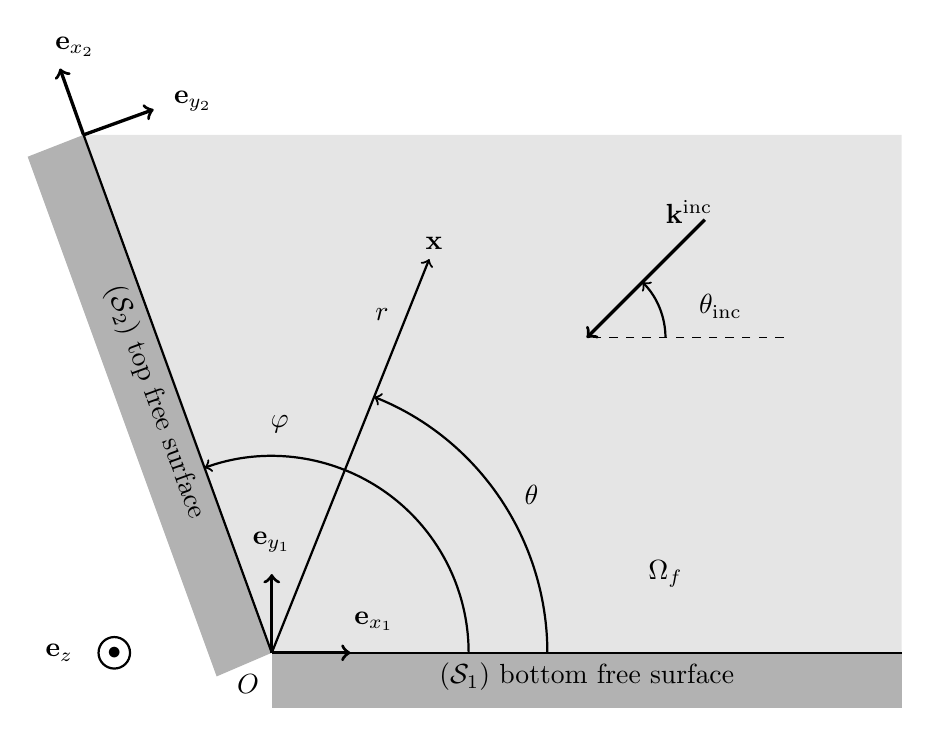
\begin{tikzpicture}
	\fill[color=gray!20] (0,0) -- (8,0)  -- (8,6.5778) -- (-2.39,6.5778) -- cycle;  
	\draw[ thick, ->] (2.5,0) arc (0:110:2.5);
	
	\fill[color=gray!60] (0,0) -- (8,0)  -- (8,-0.7) -- (0,-0.7) -- cycle;  
	
	\fill[color=gray!60] (0,0) --  (-2.39,6.5778) --(-3.1,6.3) -- (-0.7,-0.3) -- cycle; 
		
	\draw[thick, color = black]  (0,0) -- (8,0) node[midway,below] {($\mathcal{S}_1$) bottom free surface};
	
	\draw[thick, color = black]  (0,0) -- (-2.39,6.5778) node[midway,below,sloped] {($\mathcal{S}_2$) top free surface};
	
	\draw[very thick, ->] (-2.39,6.5778) -- (-2.69,7.42);
	
	\node[scale=1] at (-2.5,7.7){$\mathbf{e}_{x_2}$};
	
	\draw[very thick, ->] (-2.39,6.5778) -- (-1.5,6.9);
	
	\node at (-1,7){$\mathbf{e}_{y_2} $};
	
	
	\node at (0.1,2.9){$\varphi$} ; 
	
	\draw[very thick, ->] (0,0) -- (1,0);
	
	\node at (1.3,0.4) {$\mathbf{e}_{x_1} $};
	
	\draw[very thick, ->] (0,0) -- (0,1);
	
	\node at (0,1.4){$\mathbf{e}_{y_1} $};
	
	\node at (-2,-0.01) {$\bullet$};
	
	\draw[thick] (-2,0) circle (0.2);
	
	\node at (-2.7,0){$\mathbf{e}_{z}$};
	
	\draw[very thick, ->] (5.5,5.5) -- (4,4);
	
	\draw[dashed] (6.5,4) -- (4,4);
	
	\draw[thick, ->] (5,4) arc (0:45:1);
	
	\node at (5.7,4.4){$\theta_{\rm inc}$};
	
	\node at (5.3,5.6){ $\mathbf{k}^{\rm inc}$};
	
	\node at (-0.3,-0.4){ $O$};
	
	\node at (5,1){$\Omega_f$ };
	
	% point observation
	
	\draw[thick, ->] (0,0) -- (2,5); 
	
	\draw[thick, ->] (3.5,0) arc (0:68.2:3.5);
	
	\node at (3.3,2){$\theta$};
	
	\node at (1.4,4.3){$r$};
	
	\node at (2.06,5.2){$\mathbf{x}$};
	
	\end{tikzpicture}
	\caption
[Geometry of the problem]
{Stress-free wedge of angle $\varphi$ illuminated by a plane wave of wave vector $\mathbf{k}^{\rm inc}$.}
\label{chapter5:figure1}
\end{figure}
The dimensionless form of the problem is obtained  by defining the function $h$ by
\begin{equation}
\label{Chapter5:dimensionless}
g(\mathbf{x},t) = 2A \, e^{i \omega t} \, h(k_0 \mathbf{x}).  
\end{equation}

The dimensionless function $h$ is the sum of the  incident dimensionless  wave $h_{inc}$ and of the scattered dimensionless  wave $v$
\begin{equation}
h = h_{inc} + v
\label{decompinc}
\end{equation}
In this decomposition, the scattered wave $v$ is the sum of two fields : the Geometric-Elastodynamic (GE) field, which  is the sum of the possibly multiple specular reflections of the incident wave and of fictitious fields compensating the incident wave in shadow zones, and the diffracted field. A detailed description of the GE field, in the case of a half-plane scatterer, is given by Kamta-Djakou et al. \cite{Audrey}.

The system \eqref{Chapter5:WaveMotion}-\eqref{Chapter5:CL} is equivalent to the following  system of equations for the dimensionless problem, obtained by inserting Fourier transform \eqref{Chapter5:dimensionless} and decomposition \eqref{decompinc} into equations \eqref{Chapter5:WaveMotion} and \eqref{Chapter5:CL}
\begin{equation}
\label{Chapter5:Adimen_waveMotion}
\begin{cases}
(\triangle+1)v =  0 \quad \text{in } \Omega_f, \\
Bv =  -Bh_{inc} \quad \quad \quad \text{on } \mathcal{S}_j, \quad j=1,2
\end{cases}.
\end{equation}

In order to obtain a solution to this problem which is physically relevant, the limiting absorption principle is used. It consists in substituting the wave number $k_0$ by a complex one $k_0 e^{-i\epsilon} $ with $\epsilon > 0$. This means that absorption occurs in the medium and thus the scattered waves attenuate with the distance. The system (\ref{Chapter5:Adimen_waveMotion}) then becomes :
\begin{equation}
\label{Chapter5:waveMotion_epsilon}
(S_\epsilon^*) \quad
\begin{cases}
(\triangle+ \, e^{-2i\epsilon}) v^\epsilon  =  0 \quad \text{in } \Omega_f, \\
Bv^\epsilon  =  -Bh_{\rm inc}^\epsilon  \quad \text{on } \mathcal{S}_j, \quad j=1,2
\end{cases}
\end{equation}

The physically relevant solution to (\ref{Chapter5:Adimen_waveMotion}), called the outgoing solution, can now be defined. It is the one obtained when taking $\epsilon \to 0$ in (\ref{Chapter5:waveMotion_epsilon}). This limit is noted $v^0$. Its integral representation is found hereafter.

\subsection{Outgoing solution: integral representation}
\label{integral_representation}

First, a special class of distributions is defined.
\begin{definition}
The distribution $f\in \mathcal{A}$ if :
\begin{itemize}
\item $f \in \mathcal{S}'(\mathbb{R})$ (f is a tempered distribution)
\item supp$(f) \subset \lbrack 0,+\infty \lbrack$
\item $\exists C_0>0$ such that
$$ \sup_{-\pi<\theta<0} \int_{\rho>C_0}|\hat{f}(\rho e^{i\theta})|^2\,d\rho <\infty$$
where $\hat{f}$ is the Fourier transform of $f$ defined by $\hat{f}(\xi)=\int_{\mathbb{R}}f(x)e^{-ix\xi}\, dx$.
\item $\hat{f}(\xi)$ is holomorphic near $\xi=1$
\end{itemize}
\label{defClassA}
\end{definition}
The outgoing solution to (\ref{Chapter5:Adimen_waveMotion}) can now be defined properly.

\begin{definition}
An outgoing solution of the equation (\ref{Chapter5:Adimen_waveMotion}) is a solution v of the form 
\begin{equation}
\label{Chapter5:decomposition}
v=v_1|_{\Omega_f}+v_2|_{\Omega_f}
\end{equation}
where, for $j=1,2$ :
\begin{equation}
\label{inv_potentiels}
v_j=-\lim_{\epsilon \to 0} \left(\Delta+e^{-2i\epsilon}\right)^{-1} \left[ \alpha_j \otimes \delta_{\mathcal{S}_j} \right]
\end{equation}
$\alpha_j \in \mathcal{A}$ are unknown and $\delta_{\mathcal{S}_1}$ and $\delta_{\mathcal{S}_2}$ are the Dirac delta functions on the faces $\mathcal{S}_1$ and $\mathcal{S}_2$ of the wedge respectively (these functions verify $\delta_{\mathcal{S}_j}(x,y)=1$ on $\mathcal{S}_j$, and $\delta_{\mathcal{S}_j}(x,y)=0$ elsewhere).

\end{definition}
The following theorem is proven by Croisille and Lebeau in \cite{CroisilleLebeau} :
\begin{theorem}
The equation \eqref{Chapter5:Adimen_waveMotion} admits a unique outgoing solution.
\end{theorem}

The aim of this chapter is to extend and detail the computation of this outgoing solution for the stress-free wedge immersed in a fluid using the spectral functions method.

The double Fourier transform of a tempered distribution and its inverse are defined by :
\begin{subequations}
\begin{equation}
\hat{f}(\xi,\eta)=\int \int_{\mathbb{R}^2}f(x,y)e^{-i(x\xi+y\eta)}\, {\rm d}x {\rm d}y
\label{fourierdef}
\end{equation}
\begin{equation}
f(x,y)=\frac{1}{4\pi^2}\int\int_{\mathbb{R}^2} \hat{f}(\xi,\eta)e^{i(x\xi+y\eta)}\rm d\xi \rm d\eta
\label{invfourierdef}
\end{equation}
\label{fullfourierdef}
\end{subequations}

The double Fourier transform of (\ref{inv_potentiels}) using \eqref{fourierdef} gives
\begin{equation}
\label{Fourier}
\hat{v_j^\epsilon} =  \left[ \xi^2 + \eta^2 - e^{-2i\epsilon} \right]^{-1} \hat{\alpha_j}.
\end{equation}

 The dimensionless velocity potential $v_j^\epsilon$ is then found by applying the inverse Fourier transform in $\xi$ and $\eta$ to \eqref{Fourier}. 
\begin{equation}
\label{velocity_inv_fourier2}
v_j^\epsilon = \dfrac{1}{4\pi^2}  \int_{-\infty}^{+\infty}\left( \int_{-\infty}^{+\infty} \dfrac{e^{iy_j\eta}}{ \xi^2 + \eta^2 - e^{-2i\epsilon}} {\rm d}\eta \right)\,  \hat{\alpha_j}(\xi) \,  e^{i x_j \xi}  {\rm d} \xi.
\end{equation}

For  $\epsilon \neq 0$, the inner integrand poles are given by
\begin{equation}
 \eta = \pm \sqrt{e^{-2i\epsilon} - \xi^2}  = \pm \zeta_0^\epsilon
\end{equation} 
and are never crossed by integration along the real axis. The inner integral on $\eta$ in \eqref{velocity_inv_fourier2} can be computed using the residue theorem which leads to the following result
\begin{equation}
\label{champ_epsilon}
v_j^\epsilon(x_j,y_j) = \dfrac{i}{4\pi} \int_{-\infty}^{+\infty}  \dfrac{e^{i|y_j|\zeta_0^\epsilon(\xi)} e^{i x_j \xi}}{\zeta_0^\epsilon(\xi)} \hat{\alpha_j}(\xi) \, {\rm d}\xi.
\end{equation}
This integral is well defined if $\text{Im}(\zeta_0^\epsilon) > 0$, so that the exponential in the integral decreases with the distance $y_j$ and the absorption principle is respected. Function $\zeta_0^\epsilon(\xi)$ then satisfies for $\xi$ real
\begin{subequations}
\label{zeta_function}
\begin{align}
\zeta_0^\epsilon(\xi)&= i\sqrt{\xi^2-e^{-i\epsilon}} \quad \text{if} \quad \vert \xi\vert \geq 1,\\
\label{zeta_function_inferior1}
\zeta_0^\epsilon(\xi)&= -\sqrt{e^{-i\epsilon}-\xi^2} \quad  \text{if} \quad \vert \xi\vert \leq 1.
\end{align}
\end{subequations}
The branch points of the function $\zeta_0^\epsilon(\xi)$ are $\pm  \, e^{-i\epsilon}$ and are also poles of the integrand in \eqref{champ_epsilon}. For $\epsilon > 0$, integral \eqref{champ_epsilon} is well defined because these complex singular points are never crossed by the integration contour (the real axis). The integration contour of \eqref{champ_epsilon}, is deformed into the contour $\Gamma_0$ illustrated on Fig.~\ref{chapter5:figure2} so that these singular points $\pm  \, e^{-i\epsilon}$ are not crossed by the new contour $\Gamma_0$  when $\epsilon \rightarrow 0$ (for which the physical outgoing solution of (\ref{Chapter5:waveMotion_epsilon}) is obtained). The curved arrows on Fig.~\ref{chapter5:figure2} are described later in section \ref{Chapter5:regular_part}.

Thus, even for $\epsilon=0$, the integral
\begin{equation}
\label{champ}
v_j^0(x_j,y_j) = \dfrac{i}{4\pi} \int_{\Gamma_0}  \dfrac{e^{i|y_j|\zeta_0^0(\xi)} e^{i x_j \xi}}{\zeta_0^0(\xi)} \hat{\alpha_j}(\xi)  \, {\rm d}\xi
\end{equation}
converges.
Using \eqref{Chapter5:decomposition}, our initial solution is then
\begin{equation}
\label{initial_sol}
v(\mathbf{x}) = v_1^0(x_1,y_1) + v_2^0(x_2,y_2)
\end{equation}

\begin{figure}[ht]%
	\centering
	\begin{tikzpicture}
	\node at (0,0) {\large $\times$};
	\node at (-0.35,0.35) {\large $0$};
	\node at (2,0) {\large $\times$}; % Pole
	\node at (2,-0.35) {\large $1$};
	\node at (-2,0) {\large $\times$};
	\node at (-2,0.35) {\large $-1$}; %pole
	\node at (3.5,-0.38) {\large $(\Gamma_0)$};
	\draw[ thick, ->] (-2.5,-0.5) arc (180:235:1);
%	\node at (-2.8,-0.9) {\large $\mathcal{F}_1$};
	\draw[ thick, ->] (2.5,0.5) arc (0:45:1); %ici c'est les fleches 
	%\node at (2.8,0.9) {\large $\mathcal{F}_2$};
    \node at (4.5,0.3) {\large $\sigma$};
    \node at (-0.3,1.5) {\large $\tau$};
	\draw[step=1.5cm,gray,thick,dashed,->,>=stealth'] (-4.5,0) -- (4.5,0);
	\draw[step=1.5cm,gray,thick,dashed,->,>=stealth'] (0,-1.5) -- (0,1.5);
	\draw[very thick,black,yshift=0pt,
	decoration={ markings,  % This schema allows for fine-tuning the positions of arrows 
		mark=at position 0.1 with {\arrow{latex}},
		mark=at position 0.6 with {\arrow{latex}},
		mark=at position 0.9 with {\arrow{latex}}},
	postaction={decorate}]
	(-4,0)  -- (-2.25,0)  arc (-180:0:0.25)  -- (1.75,0)arc (180:0:0.25)  --  (4,0); % ca c'est l'axe
	\end{tikzpicture}
\caption
[Contour $\Gamma_0$]
{Integration contour $\Gamma_0$ in the complex plane $\xi = \sigma + i \tau$. The curved arrows show the deformation of $\Gamma_0$ into the imaginary axis.}
\label{chapter5:figure2}
\end{figure}

In the next section, an asymptotic evaluation of integral \eqref{champ} is conducted in order to obtain a far-field approximation of the diffracted wave. The \acrshort{gtd} diffraction coefficient is defined and its expression \eqref{GTDCoeff_SF} is given with respect to the spectral functions $\hat{\alpha}_1(\xi)$ and $\hat{\alpha}_2(\xi)$.
%One of the goals of this chapter is to compute the spectral functions $\hat{\alpha}_1(\xi)$ and $\hat{\alpha}_2(\xi)$ in order to find the GTD diffraction coefficient \eqref{GTDCoeff_SF}. 
%The accuracy of the spectral functions method is evaluated in section 4 by comparing results of \eqref{GTDCoeff_SF} with \eqref{GTDCoeff_Dir} in the case of Dirichlet boundary conditions and \eqref{GTDCoeff_Neu} in the case of Neumann boundary conditions. Section \ref{Chapter5:resolution} is devoted to the computation of the spectral functions $\hat{\alpha}_1$ and $\hat{\alpha}_2$.

\subsection{Far-field asymptotics}
\label{CoeffDiffAc}

Variable change $\xi = \cos \beta$, ${\rm d} \xi = - \sin \beta \, {\rm d}\beta$ allows us to transform \eqref{champ} for $j=1$ in
\begin{equation}
\label{face1_solution_exacte}
v_1^0(r \cos \theta,r \sin \theta) =  \dfrac{i}{4 \pi} \int_{C_0}  e^{i r (\cos \beta \cos \theta - |\sin \theta| \sin \beta)}  \hat{\alpha}_1( \cos \beta) \, {\rm d}\beta,
\end{equation}
where $C_0$ is depicted on Fig.~\ref{chapter5:figure3}. 

\begin{figure}[ht]%
\begin{center}
 \begin{tikzpicture}
\draw[step=1.5cm,gray,very thin,dashed](-1,-2.7)grid(5.7,3.7);
%\draw[thin](-1,0)-- (0,0);
\draw[thin] (-1,0)  -- (5,0) node[above]{$\sigma$};
%\drawn[thin] -- (pi+1,0) node[below]{$\sigma$};
\draw[thin](0,-2.5)--(0,3.5) node[left]{$\tau$};
\foreach \x in {pi} {  
  \draw (\x,-1pt) -- (\x,1pt) node[pos=0,above] {$\pi$};
  }

\node at (-0.2,0.2) {$0$};
\node at (0.92,0.3) {$\bar{\theta}_s$};
%\node at (3.5,-3.8) {$(\mathcal{C}_\xi)$};
\node at (3.5,-2.6) {$\mathcal{C}_0$};
\node at (1.7,-1.5) {$\gamma_0$};

\draw[black,very thick][domain=0:3.5] plot({2*pi/7 - acos(1/cosh(\x))*pi/180},\x);
\draw[black,very thick][domain=-2.8:0] plot({2*pi/7 + acos(1/cosh(\x))*pi/180},\x);
\draw[very thick,black,xshift=0pt,
decoration={ markings,  % This schema allows for fine-tuning the positions of arrows 
      mark=at position 0.8 with {\arrow{latex}}},
      postaction={decorate}]
      (0.3,-0.2) arc (270:180:0.2) -- (0.1,3); 
\draw[very thick,black,yshift=0pt,
decoration={ markings,  % This schema allows for fine-tuning the positions of arrows 
      mark=at position 0.5 with {\arrow{latex}}},
      postaction={decorate}]
      (pi-0.2,-0.2) -- (0.3,-0.2) ;
%\draw[very thick] (0.3,0) arc (270:180:0.2);

\draw[very thick,black,xshift=89.5pt,
decoration={ markings,  % This schema allows for fine-tuning the positions of arrows 
      mark=at position 0.5 with {\arrow{latex}}},
      postaction={decorate}]
      (0,-2.8) -- (0,-0.4) arc (0:90:0.2) ;
      \draw[very thick,black,
decoration={ markings,  % This schema allows for fine-tuning the positions of arrows 
      mark=at position 0.1 with {\arrow{latex}}},
      postaction={decorate}]
      (1.3988,-pi/6)  -- (0.3964,pi/6);  
\end{tikzpicture}
\end{center}
\caption
[Integration path $\mathcal{C}_0$ and the steepest descent path $\gamma_0$ in the complex plane $\beta = \sigma + i\tau$]
{Integration path $\mathcal{C}_0$ and the steepest descent path $\gamma_0$ in the complex plane $\beta = \sigma + i\tau$. $\bar{\theta}_s$ is the phase stationary point.}
\label{chapter5:figure3}
\end{figure}


Let us introduce the variable $\bar{\theta}$ defined as
\begin{equation}
\label{obs}
\bar{\theta} =
\begin{cases}
\theta \qquad \quad \; \text{if } \theta < \pi \\ 
2\pi - \theta \quad \text{if } \theta \geq \pi 
\end{cases}.
\end{equation}
Finally, using \eqref{obs} in \eqref{face1_solution_exacte}, we have
\begin{equation}
v_1^0(r \cos \theta,r \sin \theta) = \dfrac{i}{4 \pi} \int_{C_0}  e^{i r \cos ( \beta + \bar{\theta})} \hat{\alpha}_1(\cos \beta)  \, {\rm d}\beta.
\label{C2:v1ff}
\end{equation}
The same process is applied to \eqref{champ} for $j=2$ and leads to
\begin{equation}
v_2^0(r \cos (\varphi - \theta),r \sin (\varphi - \theta)) = \dfrac{i}{4 \pi} \int_{C_0}  e^{i r \cos ( \beta \, + \, \overline{\varphi - \theta})}  \hat{\alpha}_2( \cos \beta) \, {\rm d}\beta
\label{C2:v2ff}
\end{equation}
with $\overline{\varphi - \theta}$ defined in the same way as \eqref{obs}. The saddle points of the phase functions in equations \eqref{C2:v1ff} and \eqref{C2:v2ff} are respectively $\beta = \bar{\theta}_s = \pi - \bar{\theta} $ and $\beta = \bar{\theta}_s = \pi - \overline{\varphi-\theta}$. These saddle points are always in the interval $[0,\pi]$. Poles of the spectral functions $\hat{\alpha}_1$ and $\hat{\alpha}_2$ may be crossed during the deformation of contour $C_0$ into the steepest descent path $\gamma_0$ (see Fig.~\ref{chapter5:figure3}). These poles and their corresponding residues are determined in section \ref{Chapter5:sing_part}. They contribute to the integrals \eqref{champ} and lead to the geometrical field, noted $v^{(GE)}$. Their contribution can be computed using the residue theorem. The resulting integral after the contour deformation is approximated using the steepest descent method (see appendix \ref{PhaseStationnaire}). The contribution of the saddle points $  \bar{\theta}_s $ are respectively:
\begin{equation}
\label{diffracted_field1}
v_1^{0 \rm (diff)}(x_1,y_1) = \dfrac{e^{-i\frac{\pi}{4}}}{2\sqrt{2\pi}}\dfrac{e^{-ir}}{\sqrt{r}} \hat{\alpha}_1( - \cos \theta)   
\end{equation}
and
\begin{equation}
\label{diffracted_field2}
v_2^{0 \rm (diff)}(x_2,y_2) = \dfrac{e^{-i\frac{\pi}{4}}}{2\sqrt{2\pi}} \dfrac{e^{-ir}}{\sqrt{r}} \hat{\alpha}_2( - \cos ( \varphi - \theta)).   
\end{equation}
Finally in the far-field approximation, $r \gg 1$, using \eqref{initial_sol} and \eqref{diffracted_field1} - \eqref{diffracted_field2}, the total field is 
\begin{equation}
v^{\rm tot} = v^{\rm (GE)} + v^{\rm diff}
\end{equation}
where $v^{diff}$ is the field diffracted by the wedge edge
\begin{equation}
\label{Chapter5:diff_field}
v^{ diff} = \dfrac{e^{-i\frac{\pi}{4}}}{2\sqrt{2\pi}} \dfrac{e^{-ir}}{\sqrt{r}} [\hat{\alpha}_1( - \cos \theta) + \hat{\alpha}_2( - \cos ( \varphi - \theta))].
\end{equation}
Using \eqref{Chapter5:dimensionless} and \eqref{Chapter5:diff_field}, the \acrshort{gtd} diffraction coefficient is defined as
\begin{equation}
\label{GTDCoeff_SF}
D^{GTD} = \dfrac{e^{-i\frac{\pi}{4}}}{2\sqrt{2\pi}} \, [\hat{\alpha}_1( - \cos \theta) + \hat{\alpha}_2( - \cos ( \varphi - \theta))]
\end{equation}
where $\hat{\alpha}_1$ and $\hat{\alpha}_2$ are unknown spectral functions. 

One of the aims of this chapter is to compute the spectral functions $\hat{\alpha}_1(\xi)$ and $\hat{\alpha}_2(\xi)$ in order to find the \acrshort{gtd} diffraction coefficient \eqref{GTDCoeff_SF}. The accuracy of the spectral functions method is then evaluated by comparing results of \eqref{GTDCoeff_SF} with analytic expressions \eqref{GTDCoeff_Dir} in the case of Dirichlet boundaries and \eqref{GTDCoeff_Neu} in the case of Neumann boundaries. Section \ref{Chapter5:resolution} is devoted to the computation of the spectral functions $\hat{\alpha}_1$ and $\hat{\alpha}_2$.

\section{Spectral functions computation}
\label{Chapter5:resolution}

To compute the spectral functions, the functional equations satisfied by these spectral functions $\hat{\alpha}_1$ and $\hat{\alpha}_2$ first have to be determined.
\subsection{Functional equations of spectral functions}
\label{C2:functional_system}

The velocity potential in the boundary conditions of the system \eqref{Chapter5:waveMotion_epsilon} is substituted by its expression \eqref{initial_sol}. It then leads to the following system of equations for the boundary conditions on each wedge face:
\begin{equation}
\label{CL}
\begin{cases}
Bv_1^0(x_1,0) + Bv_2^0(x_2 \cos \varphi,x_2 \sin \varphi)  =  -Bv^0_{\rm inc} \mid_{\mathcal{S}_1}\\
Bv_1^0(x_1 \cos \varphi,x_1 \sin \varphi) + Bv_2^0(x_2,0)   =  -Bv^0_{\rm inc} \mid_{\mathcal{S}_2}
\end{cases}.
\end{equation}
The Fourier transform is applied to the potential velocity expression on the face of each wedge
\begin{align}
\mathcal{F}(x_j \mapsto v_j^0 (x_j,0))(\xi) & =  \dfrac{i}{4\pi} \int_{\Gamma_0}  \dfrac{\hat{\alpha_j}(\lambda)}{\zeta_0^0(\lambda)}  \left( \int_0^{\infty} \, e^{-i x_j (\xi-\lambda)} dx_j \right) {\rm d} \lambda,\\
& =  \dfrac{1}{4\pi} \int_{\Gamma_0} \dfrac{\hat{\alpha_j}(\lambda)}{\zeta_0^0(\lambda) (\xi - \lambda)} {\rm d} \lambda \nonumber
\end{align}
and
\begin{align}
\mathcal{F} \left( x_j \mapsto v_j^0 \left( x_j \cos \varphi,x_j \sin \varphi \right) \right)(\xi)  & =  \dfrac{i}{4\pi} \int_{\Gamma_0}  \dfrac{\hat{\alpha_j}(\lambda)}{\zeta_0^0(\lambda)}  \left( \int_0^{\infty} \, e^{-i x_j \left( \xi - \lambda  \, \cos \varphi - |\sin \varphi| \, \zeta_0^0(\lambda) \right)} dx_j \right) {\rm d} \lambda,\\
& = \dfrac{1}{4\pi} \int_{\Gamma_0} \dfrac{ \hat{\alpha_j}(\lambda)}{\zeta_0^0(\lambda) \left[ \xi - \lambda \, \cos \varphi  - |\sin \varphi| \, \zeta_0^0(\lambda) \right]} {\rm d} \lambda.  \nonumber
\end{align}
The potential velocity's normal derivative on the face of each wedge is computed using \eqref{champ}, and by noting that for each face $n_j=y_j$ (see Fig.~\ref{chapter5:figure1}) :
\begin{equation}
\frac{\partial v_j^0}{\partial n_j}(x_j,y_j) = -\frac{1}{4\pi} \int_{\Gamma_0} te^{i\xi x_j}e^{i|y_j|\zeta_0^0(\xi)} \hat{\alpha_j}(\xi)\, d\xi,
\end{equation}
where $t= \rm sgn \, y_j$. In order to go from one Cartesian coordinate system to another, the following change in variables is given for $j=1,2$ (see Fig.~\ref{chapter5:figure1}) :
\begin{eqnarray}
\label{changecoords}
\left\{
\begin{array}{l}
x_{3-j}=x_j\cos\varphi+y_j\sin\varphi \\
y_{3-j}=x_j\sin\varphi-y_j\cos\varphi
\end{array}
\right.
\end{eqnarray}
This yields :
\begin{align}
\frac{\partial v_j^0}{\partial n_{3-j}}&=\frac{\partial v_j^0}{\partial y_{3-j}}= \sin\varphi \frac{\partial v_j^0}{\partial x_j}-\cos\varphi \frac{\partial v_j^0}{\partial y_j}\\
&=-\frac{1}{4\pi}\int_{\Gamma_0}\frac{(\xi\sin\varphi-t\cos\varphi\zeta_0^0(\xi))}{\zeta_0^0(\xi)}e^{i(\xi x_j+|y_j|\zeta_0^0(\xi))}\hat{\alpha_j}(\xi)\,d\xi
\end{align}
The Fourier transform can now also be applied to the potential velocity's normal derivative on the each face of the wedge
\begin{align}
\mathcal{F}(x_j \mapsto \frac{\partial v_j^0}{\partial n_j} (x_j,0))(\xi)&=-\frac{1}{4\pi} \int_{\Gamma_0}  \hat{\alpha_j}(\lambda)\left( \int_0^{\infty} \, e^{-i x_j (\xi-\lambda)} dx_j \right)\, d \lambda \nonumber\\
&=\frac{i}{4\pi}\int_{\Gamma_0}\frac{\hat{\alpha_j}}{\xi-\lambda}\, d\lambda
\end{align}
and
\begin{align}
\mathcal{F} &\left( x_j \mapsto \frac{\partial v_j^0}{\partial n_{3-j}} ( x_j \cos \varphi,x_j \sin \varphi) \right)(\xi)  \nonumber\\
& =  -\frac{1}{4\pi} \int_{\Gamma_0}  \frac{(\lambda\sin\varphi-t\cos\varphi\zeta_0^0(\lambda))}{\zeta_0^0(\lambda)}\hat{\alpha_j}(\lambda)  \left( \int_0^{\infty} \, e^{-i x_j \left( \xi - \lambda  \, \cos \varphi - |\sin \varphi| \, \zeta_0^0(\lambda) \right)} dx_j \right) \,d \lambda, \nonumber\\
& = \frac{i}{4\pi} \int_{\Gamma_0} \dfrac{ \lbrack \lambda\sin\varphi-t\cos\varphi\zeta_0^0(\lambda)\rbrack \, \hat{\alpha_j}(\lambda)}{\zeta_0^0(\lambda) \left[ \xi - \lambda \, \cos \varphi  - |\sin \varphi| \, \zeta_0^0(\lambda) \right]} \, d\lambda,
\end{align}
here $t=\rm sgn \sin \varphi$.

The dimensionless incident wave on the faces $\mathcal{S}_1$ and $\mathcal{S}_2$ of the wedge which is involved at the right side of \eqref{CL} is respectively:
\begin{subequations}
\label{CL2}
\begin{align}
v^0_{\rm inc}(x_1,y_1) & =  \dfrac{1}{2} \, e^{i \, (x_1 \cos \theta_{inc}+y_1\sin\theta_{inc} ) } ,\\
v^0_{\rm inc}(x_2,y_2) & =   \dfrac{1}{2} \, e^{i \, (x_2 \cos (\varphi - \theta_{inc} )+y_2\sin(\varphi-\theta_{inc}))} 
\end{align}
\end{subequations}

Therefore, applying the Fourier transform to \eqref{CL} leads to the following functional system of equations:
\begin{equation}
\label{functional_eq}
\begin{cases}
DM(\hat{\alpha}_1)(\xi) + TM(\hat{\alpha}_2)(\xi) = \dfrac{W_1}{\xi - Z_1} \\
TM(\hat{\alpha}_1)(\xi) + DM(\hat{\alpha}_2)(\xi)  = \dfrac{W_2}{\xi - Z_2} 
\end{cases}
\end{equation}
where $Z_1 =  \cos \theta_{\rm inc}$, $Z_2 =  \cos (\varphi - \theta_{\rm inc})$, $W_1=W_2=1$ in the case of Dirichlet boundary conditions and $W_1=\sin\theta_{inc}, \quad W_2=\sin(\varphi-\theta_{inc})$ in the case of Neumann boundary conditions. $DM$ is an integral operator defined as
\begin{equation}
\label{DM_operator}
\begin{split}
DM(\hat{\alpha}_1)(\xi) = \int_{\Gamma_0} DM(\xi,\lambda) \, \hat{\alpha}_1(\lambda) \, d \lambda =\dfrac{1}{2i\pi} \int_{\Gamma_0} \dfrac{dm(\lambda)  }{\xi - \lambda} \hat{\alpha}_1(\lambda) \, d\lambda
\end{split}
\end{equation}
where 
\begin{equation}
\label{dmDir}
dm(\lambda) = \dfrac{1}{\zeta_0^0(\lambda)}
\end{equation}
in the case of Dirichlet boundary conditions and 
\begin{equation}
\label{dmNeu}
dm(\lambda)=1
\end{equation}
in the case of Neumann boundary conditions. 

$TM$ is an integral operator defined as
\begin{equation}
\label{TM_operator}
\begin{split}
TM(\hat{\alpha}_1)(\xi) &= \int_{\Gamma_0} TM(\xi,\lambda) \, \hat{\alpha}_1(\lambda) \, {\rm d} \lambda =\dfrac{1}{2i\pi} \int_{\Gamma_0} \dfrac{ tm(\lambda)}{ \xi- \lambda \cos \varphi  - |\sin \varphi| \zeta_0^0(\lambda)} \hat{\alpha}_1(\lambda) \, {\rm d} \lambda 
\end{split}
\end{equation}
where 
\begin{equation}
\label{tmDir}
tm(\lambda)=\dfrac{1}{\zeta_0^0(\lambda)}
\end{equation}
in the case of Dirichlet boundary conditions and 
\begin{equation}
\label{tmNeu}
tm(\lambda)=\dfrac{\lambda\sin\varphi-t\cos\varphi\zeta_0^0(\lambda)}{\zeta_0^0(\lambda)}
\end{equation}
in the case of Neumann boundary conditions.
Note that the function $TM$ can be expressed as
\begin{equation}
TM(\xi,\lambda) =  \dfrac{1}{2i\pi} \dfrac{ tm(\lambda)}{ \xi- T_0(\lambda)} , 
\end{equation}
where, applying the variable change $\lambda=\cos\theta$
\begin{equation}
\label{Trans_operator}
T_0(\lambda=\cos\theta) =  \lambda \cos \phiti  + \sin \phiti \, \zeta_0^0(\lambda) =  \cos (\theta + \phiti)
\end{equation}
with 
\begin{equation}
\phiti =
\begin{cases}
 \varphi \quad \text{if} \quad 0 < \varphi < \pi \qquad \\
 2\pi - \varphi \quad \text{if} \quad \pi < \varphi < 2\pi
 \label{phitilde}
\end{cases}
\end{equation}
Function $T_0$ is therefore called the translation operator, since it translates the complex angle $\theta$ to $\theta+\phiti$. By using this angular variable $\phiti$, defined differently for wedge angles lower and higher than $\pi$, the description of the spectral functions method can be written the same way for wedge angles $\varphi$ lower and higher than $\pi$, even if the final results (the diffraction coefficients) are different for wedge angles $\pi<\varphi<2\pi$ and $2\pi-\varphi$. Indeed, the variable $\varphi$ appears in all the resolution (for example, it appears in the expression of pole $Z_2$), whereas the variable $\phiti$ appears only in the definition of the function $T_0$ in \eqref{Trans_operator} and of the domain $\Omega_0$ in which $T_0$ operates, defined as
\begin{equation}
\label{Domain_Omega0}
\Omega_0 =\{\xi\in\mathbb C, \ \xi=\cos \theta, \ 0< {\rm Re } \, \theta < \pi -\phiti \}.
\end{equation}
Domain $\Omega_0$ is delineated by the hyperbola 
\begin{equation}
\partial \Omega_0^+ = \{   \xi \in \mathbb{C}, \quad \xi = \cos \theta, \quad {\rm Re}  \theta = \pi - \phiti \}.
\end{equation}
Domain $\Omega_0$ and its upper boundary $\partial \Omega_0^+$ are illustrated on Fig.~\ref{chapter5:figure4}. Domain $\Omega_0$ is the grey area in Fig.~\ref{chapter5:figure4}.

\begin{figure}[h]
\centering
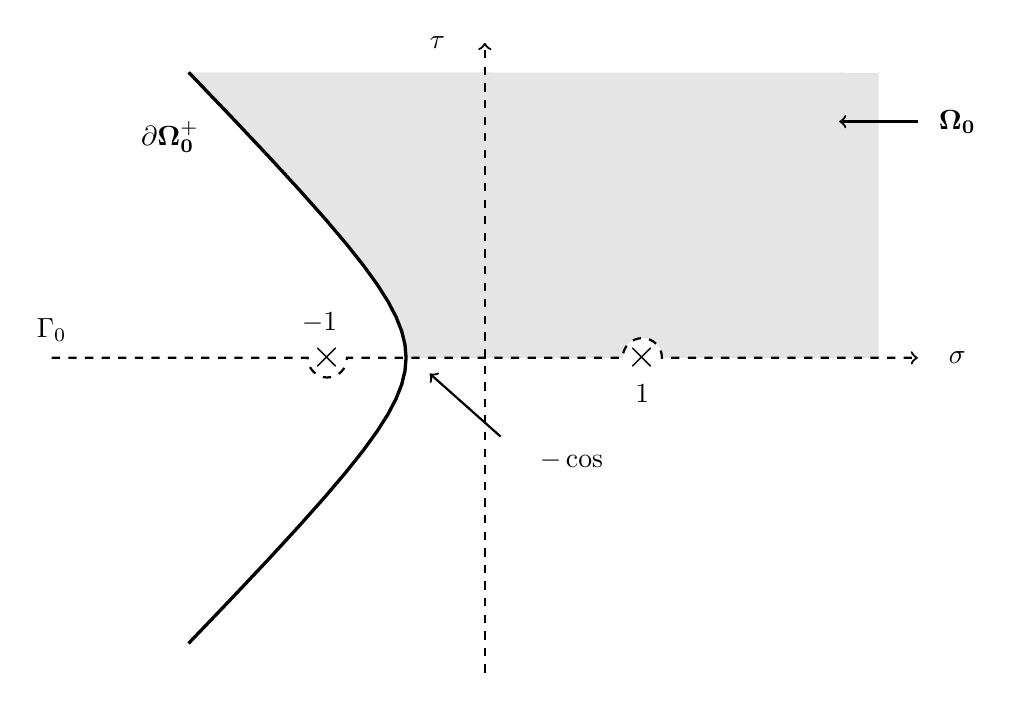
\begin{tikzpicture}
% Filling Omega_0
\fill [color=gray!20]
(5,0)
-- plot [domain=0:2] ({-cosh(\x)},{sinh(\x)})
-- (5,3.62)
-- cycle;

\fill[color=white] (2,0) circle (0.25);

\node at (2,0) {\Large $\mathbf{\times}$}; % Pole
\node at (2,-0.45) { $1$};
\node at (-2,0) {\Large $\mathbf{\times}$};
\node at (-2.1,0.45) {$-1$}; %pole
\node at (-5.5,0.35) {$\Gamma_0$};
\draw[dashed,thick, ->]
      (-5.5,0) -- (-2.25,0)  arc (-180:0:0.25)  -- (1.75,0)arc (180:0:0.25) -- (5.5,0);
\draw[dashed,thick,->]
	  (0,-4) -- (0,4);
\node at (6,0) {$\sigma$};
\node at (-0.6,4) { $\tau$};
      % axis

%% arrows indicating countour deformation
%\draw[ thick, ->] (-3,-0.25) arc (180:235:1);
%\node at (-3.2,-0.9) {$\mathcal{F}_1$};
%\draw[ thick, ->] (4.0,0.3) arc (0:45:1); 
%\node at (4.5,0.8) { $\mathcal{F}_2$};

% Hyperbola (contour  partial_Omega_0 )
\draw[black, very thick][domain=-2:2] plot({-cosh(\x)}, {sinh(\x)});
\node at (-4.0,2.8) { $\mathbf{\partial \Omega_0^+}$};
\draw[thick,->] (0.2,-1.0)--(-0.7,-0.2);
\node at (1.1,-1.3) {$-\cos \phiti$};

%  Omega_0
\draw [thick, ->] (5.5,3)--(4.5,3);
\node at (6,3) {$\mathbf{\Omega_0}$};

\end{tikzpicture}
\caption
[Contour $\partial \Omega_0^+$]
{Domain $\Omega_0$ (the grey area) and its upper boundary $\partial \Omega_0^+$ in the complex plane $\xi=\sigma+i\tau$. The lower boundary of $\Omega_0$ is the semi-axis $[-\cos \phiti,+\infty[$.}
\label{chapter5:figure4}
\end{figure}
Having found the system of functional equations, it is now resolved following the methodology of Croisille and Lebeau \cite{CroisilleLebeau}.

\subsection{System resolution}
\label{Chapter5:System_resolution}

The resolution of the system of functional equations \eqref{functional_eq} is necessary in order to find the values of the spectral functions $\hat{\alpha}_1 $ and $\hat{\alpha}_2 $. With these values, the diffraction coefficients can be computed using equation \eqref{GTDCoeff_SF}. 

It is shown in \cite{CroisilleLebeau} that the actions of $DM$ and $TM$ integral operators onto a singular function are constituted of a "singular term" and of a "regular term". For a singular function 
\begin{equation}
\label{Chapter5:arbitrary_function}
\phi(\xi) = \dfrac{1}{\xi - z},  \quad z \in \mathbb{C}\setminus ]-\infty,-1] \text{ with } {\rm Im} \, z \geqslant 0,
\end{equation}
contour $\Gamma_0$ is deformed into contour $\Gamma_1$ (thus crossing the whole upper half of the complex plane, as illustrated in Fig.~\ref{chapter5:figure5}) in integral operator $DM$ defined by \eqref{DM_operator}, and into contour $\partial \Omega_0^+$ (thus crossing sub-domains $\Omega_0$ and $Im\xi<0, \xi \notin \Omega_0$ as illustrated in Fig.~\ref{chapter5:figure4}) in integral operator $TM$ defined by \eqref{TM_operator}. Using the residue theorem, the result can be decomposed as
\begin{subequations}
\label{Int_op_decomp}
\begin{align}
\label{Int_op_decomp_DM}
DM(\phi)(\xi) &= \int_{\Gamma_0} DM(\xi,\lambda) \cdot \dfrac{1}{\lambda - z} \, d \lambda = \dfrac{dm(z)}{\xi - z}  + D_p(\xi,z) \\
\label{Int_op_decomp_TM}
TM(\phi)(\xi) &= \int_{\Gamma_0} TM(\xi,\lambda) \cdot \dfrac{1}{\lambda - z} \, d \lambda = \dfrac{tm(z) }{\xi - T_0(z)} 1_{\Omega_0}(z) + T_p(\xi,z),
\end{align}
\end{subequations}
where the function $T_0$ is defined in \eqref{Trans_operator} and where
\begin{equation}
1_{\Omega_0}(z) = 
\begin{cases}
1 \quad \text{if } z  \in \Omega_0, \\
0 \quad \text{else}
\end{cases}
\end{equation}
and integrals $D_p$ and $T_p$ are the regular terms, expressed as
\begin{subequations}
\label{holomorphic_functions}
\begin{align}
\label{defDp}
D_p(\xi,z) &= \dfrac{1}{2\pi i}\int_{\Gamma_1} \dfrac{dm(\lambda)}{\xi-\lambda} \cdot \dfrac{1}{\lambda - z} d\lambda, \\
\label{defTp}
T_p(\xi,z) &= \dfrac{1}{2\pi i}\int_{\partial \Omega_0^+}  \dfrac{tm(\lambda)}{\xi-T_0(\lambda)} \cdot \dfrac{1}{\lambda - z} d\lambda.
\end{align}
\end{subequations}
Croisille and Lebeau \cite{CroisilleLebeau} proved that $D_p(z,\cdot)$ and $T_p(z,\cdot)$ belong to a special class of functions $\mathcal{H}$ defined hereafter
\begin{definition}
\label{defHpl}
$H^+$ is the space of functions f which are analytical in $\{z \in \mathbb{C}, \; \mbox{Im} z <0\}$  and verify :
\begin{equation}
\underset{c>0}{sup} \int_{-\infty}^{+\infty} |f(x-ic)|^2\,dx<+\infty
\end{equation}
\end{definition}
\begin{definition}
\label{defH}
$\mathcal{H}$ is the space of the functions f analytical in $\mathbb{C}\backslash \rbrack -\infty,-1\rbrack$ such that $\forall \epsilon \in \rbrack0,\pi \lbrack, f(e^{i\epsilon} \cdot)\in H^+$.
\end{definition}

\begin{figure}[ht]
\centering
\begin{tikzpicture}
\node at (-0.5,0) {  $\times$};
\node at (-0.7,-0.35) { $0$};
\node at (1,0) { $\times$}; % Pole
\node at (1,-0.36) { $1$};

\node at (-2,0) { $\times$};
\node at (-2,0.36) {  $-1$}; %pole
\node at (-3,-0.5) { $\Gamma_1$};

\draw[dashed, decoration={markings,
 mark=at position 1.0 with {\arrow{latex}}},
      postaction={decorate}] (-1.5,0) -- (0.75,0) arc (180:0:0.25)-- (2.5,0);
\node at (3,0) {$\sigma$};
\draw[dashed, decoration={markings,
 mark=at position 1.0 with {\arrow{latex}}},
      postaction={decorate}] (-0.5,-1.5) -- (-0.5,2);
\node at (-0.8,2) {$\tau$};      

\node at (2.5,-0.4) {$(\Gamma_0)$};
      
\draw[ thick, ->] (0.75,0.5) arc (0:135:1); 
  

\draw[very thick, black, yshift=0pt,
decoration={ markings,  % This schema allows for fine-tuning the positions of arrows 
      mark=at position 0.1 with {\arrow{latex}},
      mark=at position 0.9 with {\arrow{latex}}},
      postaction={decorate}]
      (-4,0) -- (-2.25,0)  arc (-180:0:0.25) -- (-1.75,0) arc(-90:90:0.5)  -- (-4,1);
\end{tikzpicture}
\caption
[Contour $\Gamma_1$]
{Contour $\Gamma_1$. The curved arrow shows the deformation of $\Gamma_0$ (dashed line) into $\Gamma_1$.}
\label{chapter5:figure5}
\end{figure}

In the sequel, using the decomposition of the $DM$ and $TM$ operators for a function of the form of \eqref{Chapter5:arbitrary_function}, it will be shown that the unknown spectral functions $\hat{\alpha}_1$ and $\hat{\alpha}_2$ in the system \eqref{functional_eq} have a singular part. The first step for the resolution of the system \eqref{functional_eq} is then to determine this singular part.

\subsubsection{Singular part}
\label{Chapter5:sing_part}

It is well known that poles of the spectral functions lead to the reflections of the incident field on the wedge faces (these reflections can be multiple), and to the fictitious fields that compensate the incident wave in the shadow zones. The sum of these reflections with the fictitious compensating fields constitute the aforementioned GE field. The singular part of the spectral functions contains these poles. The goal of this subsection is to calculate the poles and the corresponding residues and then to determine the expression of the singular part of the spectral functions, by employing a recursive algorithm. 

Knowing the incident field on the wedge faces, which corresponds to the right-hand side of system \eqref{functional_eq}, the spectral function  $\hat{\alpha}_j$ can be written as
\begin{equation}
\label{Chapter5:ini_pol_propag}
\hat{\alpha}_j(\xi) = \dfrac{V_j}{\xi - Z_j} + X_j'(\xi), \quad j=1,2
\end{equation}
where $Z_1,Z_2$ are the initial poles, given in \eqref{functional_eq} with unknown residues $V_1$ and $V_2$ and the functions $X_j'$ are unknown, $j=1,2$. Replacing \eqref{Chapter5:ini_pol_propag} in \eqref{Int_op_decomp_DM}, it is found that
\begin{equation}
\label{Chapter5:pole_propag_DM_1}
DM(\hat{\alpha}_j)(\xi) = \dfrac{dm(Z_j) \cdot V_j}{\xi - Z_j} + D_p(\xi,Z_j)\cdot V_j + DM( X_j')(\xi).
\end{equation}
By choosing $V_j =  dm^{-1}(Z_j).W_j$, the right hand side of the system \eqref{functional_eq} is suppressed by the first term in the right hand side of \eqref{Chapter5:pole_propag_DM_1}. A new version of the system can be written on a single line with new unknown functions $X'_j, \, j=1,2$ :
\begin{equation}
DM  (X_j' )(\xi)+ TM (X_{3-j}' )(\xi) = - TM  \left(  \dfrac{V_{3-j}}{\xi - Z_{3-j}} \right) (\xi)  - D_p(V_j,Z_j)(\xi) \qquad j=1,2
\end{equation}
Applying \eqref{Int_op_decomp_TM} yields
\begin{equation}
\label{Chapter5:pol_propag_step3}
TM  \left(  \dfrac{V_j}{\xi - Z_j} \right)(\xi) = \dfrac{tm(Z_j) \cdot V_j}{\xi - T_0(Z_j)}  \, 1_{\Omega_0}(Z_j) + T_p(\xi,Z_j)\cdot V_j \qquad j=1,2
\end{equation}
Thus, $X_j'$ has a pole at $\xi = Z_j^{(1)} = T_0(Z_{3-j})$ if $Z_{3-j} \in \Omega_0$. The wave incident on face $\mathcal{S}_{3-j}$ is reflected. This reflected wave is incident on face $\mathcal{S}_j$, generating a new pole $Z_j^{(1)}=T_0(Z_{3-j})$. 
The unknown function $X_j'$ in \eqref{Chapter5:ini_pol_propag} is then decomposed as
\begin{equation}
\label{Chapter5:pol_propag_step2}
X_j'(\xi) =  \dfrac{V_j^{(1)}}{\xi - Z_j^{(1)}} + X_j''(\xi), \quad j=1,2
\end{equation}
where the function $ X_j''$ is unknown. 
Once again, the residues $V_j^{(1)}$ of these generated poles $Z_j^{(1)}$ are chosen so that they cancel the singular term in $DM(X_j')(\xi)$, found using formula \eqref{Int_op_decomp_DM}, compensating the singular term in the $TM$ operator in \eqref{Chapter5:pol_propag_step3}.

This pole propagation process is applied recursively in order to determine all the poles of the spectral functions $\hat{\alpha}_j$. This process stops when the generated poles are no longer in the domain $\Omega_0$ defined in \eqref{Domain_Omega0}. All the generated poles then belong to $\Omega_0$. 

At the end of this process, the spectral functions have the following decomposition
\begin{equation}
\label{spec_decomp}
\hat{\alpha}_j=Y_j+X_j, 
\end{equation}
where  $Y_j$ is the singular part, $X_j$ is the regular part  and $j=1,2$ is the face index. The singular part is expressed as
\begin{equation}
\label{sing_part}
 Y_j(\xi) = \sum_i \dfrac{{V_j^{(i)}}}{{\xi - Z_j^{(i)}}},
\end{equation}
where $i \in \mathbb{N}$, $Z_j^{(0)} = Z_j$ is the initial pole on each face of the wedge, $V_j^{(0)}=V_j$ is the corresponding initial residue on each face of the wedge, both linked to the incident field as expressed in \eqref{functional_eq},
\begin{equation}
\label{Generated_poles}
Z_j^{(i+1)} = T_0(Z_{3-j}^{(i)}) \quad j=1,2
\end{equation} 
are the different generated poles with their respective residues 
\begin{equation}
\label{Generated_residues}
V_j^{(i+1)}=-dm^{-1}(T_0(Z_{3-j}^{(i)})) \,  tm(Z_{3-j}^{(i)})) \, V_{3-j}^{(i)} \, 1_{\Omega_0}(Z_{3-j}^{(i)}), \quad  j=1,2.
\end{equation}
\paragraph{}
Figure \ref{poles} represents the generated poles in the complex plane for two different cases : figure \ref{poles80} for a wedge of angle $\varphi=80^o$ with an incident angle of $\theta_{inc}=55^o$ and figure \ref{poles20} for $\varphi=20^o$ and $\theta_{inc}=15^o$. As the wedge angle decreases, the number of poles increases, some poles being very close to one another, rendering the method less accurate for very small wedge angles.
\begin{figure}[h]
	\centering
	\begin{subfigure}[b]{0.4\textwidth}
	\begin{tikzpicture}[scale=2]
	\draw[->,>=stealth'] (-1.25,0) -- (1.25,0);
	\draw[->,>=stealth'] (0,-0.5) -- (0,0.5);
	\node at (1.25,0)[right]{Re};
	\node at (0,0.5)[right]{Im};
	
	\node at (-1,0){$\bullet$};
	\node at (1,0){$\bullet$};
	\draw (-1,0) node[below] {$-1$};
	\draw (1,0) node[below] {$1$};
	
	\node at ( 0.573576450    ,  0.00000000    ){$\times$};
	\node at ( 0.906307757    ,  0.00000000    ){$\times$};
	\node at (-0.258819222    ,  0.00000000    ){$\times$};
	\node at (-0.707106829    ,  0.00000000    ){$\times$};
	\end{tikzpicture}
	\subcaption{$\varphi=80^o, \, \theta_{inc}=55^o$}
    \label{poles80}
	\end{subfigure}
\hspace{1em}
\begin{subfigure}[b]{0.4\textwidth}
\begin{tikzpicture}[scale=2]
\draw[->,>=stealth'] (-1.25,0) -- (1.25,0);
\draw[->,>=stealth'] (0,-0.5) -- (0,0.5);
\node at (1.25,0)[right]{Re};
\node at (0,0.5)[right]{Im};

\node at ( 0.965925813    ,  0.00000000    ){$\times$};
\node at ( 0.996194720    ,  0.00000000    ){$\times$};
\node at ( 0.906307876    ,  0.00000000    ){$\times$};
\node at ( 0.819151998    ,  0.00000000    ){$\times$};
\node at ( 0.573576331    ,  0.00000000    ){$\times$};
\node at ( 0.707106948    ,  0.00000000    ){$\times$};
\node at ( 0.422618449    ,  0.00000000    ){$\times$};
\node at ( 0.258818895    ,  0.00000000    ){$\times$};
\node at ( -8.71558934E-02,  0.00000000    ){$\times$};
\node at (  8.71559381E-02,  0.00000000    ){$\times$};

\node at (-1,0){$\bullet$};
\node at (1,0){$\bullet$};
\draw (-1,0) node[below] {$-1$};
\draw (1,0) node[below] {$1$};
\end{tikzpicture}
\subcaption{$\varphi=20^o, \, \theta_{inc}=15^o$}
\label{poles20}
\end{subfigure}
\caption{Poles generated by the recursive algorithm plotted in the complex plane}
\label{poles}
\end{figure}

The second step of the system resolution is the determination of the regular part $X_j$ of the spectral function $\hat{\alpha}_j$, see Eq.~\eqref{spec_decomp}. The regular part is determined by using the Galerkin collocation method. Section \ref{Chapter5:regular_part} gives the principal steps of this resolution method. 

\subsubsection{Regular part}
\label{Chapter5:regular_part}

After the determination of the singular part of the solution using the pole propagation process explained in section \ref{Chapter5:sing_part}, the remaining system \ref{functional_eq} is by construction
\begin{equation}
\label{sys_regular}
\begin{cases}
DM(X_1)(\xi) + TM(X_2)(\xi) = -\underset{k}{\sum} \Big( D_p(\xi,Z_1^{(k)})\cdot V_1^{(k)}+ T_p(\xi,Z_2^{(k)})\cdot V_2^{(k)}\Big)\\
TM(X_1)(\xi) + DM(X_2)(\xi)  =  -\underset{k}{\sum} \Big( T_p(\xi,Z_1^{(k)})\cdot V_1^{(k)}+ D_p(\xi,Z_2^{(k)})\cdot V_2^{(k)}\Big)
\end{cases}
\end{equation}
where $X_j$, $j=1,2$ are the regular parts of the spectral functions \eqref{spec_decomp}, $D_p$ and $T_p$ functions are defined in \eqref{holomorphic_functions} and $Z_j^{(k)}$ are the poles of spectral function $\hat{\alpha}_j$  and their respective residues are $V_j^{(k)}$. According to Croisille and Lebeau \cite{CroisilleLebeau}, $D_p$ and $T_p$ are holomorphic on $\mathbb{C}\setminus  ]-\infty,-1]$ and therefore functions $X_1$ and $X_2$ are also holomorphic on this domain.

The functions $X_j(\xi)$, being holomorphic on $\mathbb{C}\setminus  ]-\infty,-1]$, can be approached in the vectorial subspace generated by $\varphi_k, \, 1 \leq k \leq N$ where
\begin{equation}
\label{Gal_basis}
\varphi_k(\xi) = \dfrac{d_k}{\xi + a_k}, \quad a_k \in [1,\infty[, \quad d_k=\sqrt{\frac{a_k}{\pi}}.
\end{equation}
The approximation of the solution $X_j(\xi)$ in this subspace of finite dimension is called a Galerkin approximation.

In the following, the integration contour $\Gamma_0$ pictured on Fig.~\ref{chapter5:figure2} is deformed into the imaginary axis. If $f(\lambda)$ is a holomorphic function on $\mathbb{C}\setminus  ]-\infty,-1]$, the function $\tilde f (y)=f(iy)$ is introduced so that $\tilde f$ is holomorphic on $\mathbb{C}\setminus i [1,\infty[ $. The variable change $\lambda = iy$ gives a new basis
\begin{equation}
\label{Galerkin_basis}
e_{a_k}(y) = \dfrac{d_k}{y-i{a_k}}=i\tilde \varphi_k(y), \quad \text{with} \quad d_k=\sqrt{\frac{a_k}{\pi}} \quad \text{and} \quad a_k \in [1,\infty[,
\end{equation}

Having an approximation basis of the regular part of the spectral functions, $X_j(\xi)$ can be expressed as
\begin{equation}
\label{regular_part_decomp}
X_j(\xi) \approx \sum_{k=1}^N \tilde{X}_j^k \, \varphi_k(\xi), \quad \tilde{X}_j^k \in \mathbb{C}.
\end{equation}
The coordinates $\tilde{X}_j^k$ are unknown. The system \eqref{sys_regular} then becomes, for $j=1,2$
\begin{equation}
\label{sys_regular_gal}
\sum_{k=1}^N \left[ \tilde{X}_j^k \, \int_{\Gamma_0} DM(\xi,\lambda) \varphi_k(\lambda) \, {\rm d} \lambda + \tilde{X}_{3-j}^k \, \int_{\Gamma_0} TM(\xi,\lambda) \varphi_k(\lambda) \, {\rm d} \lambda \right] = u_j(\xi), 
\end{equation}
where
\begin{equation}
\label{second_member}
u_j(\xi) = -\sum_k \Big( D_p(\xi,Z_j^k)\cdot V_j^k+ T_p(\xi,Z_{3-j}^k)\cdot V_{3-j}^k\Big) \qquad j=1,2
\end{equation}
The variable changes $\lambda = iy$ and $\xi = ix$ in \eqref{sys_regular_gal} lead to the following system $(j=1,2)$
\begin{equation}
\label{sys_regular_gal_def}
\sum_{k=1}^N \left[ \tilde{X}_j^k \, \int_{-\infty}^\infty  \widetilde{DM}(x,iy) \, e_{a_k}(y) {\rm d} y + \tilde{X}_{3-j}^k \, \int_{-\infty}^\infty  \widetilde{TM}(x,iy) \, e_{a_k}(y) {\rm d} y \right] = \tilde u_j(x) \\
\end{equation}
where $\widetilde{DM}(x,iy) = DM(ix,iy)$ and $\widetilde{TM}(x,iy) = TM(ix,iy)$. Following \cite{CroisilleLebeau}, we introduce another subspace of finite dimension in $L^2(\mathbb{R})$ which is generated by vectors $e_{b_k}$ with
\begin{equation}
\label{points_collocation}
e_{b_k}(y)=\frac{d_k}{y-ib_k}, \quad  \rm Re (b_k) \in [1,\infty[  \quad \text{and}  \quad {\rm Im} (b_k) = 0^-.
\end{equation}

Points $b_k$ are called collocation points.  The system \eqref{sys_regular_gal_def} is projected in this subspace using the following relation, for an arbitrary regular function $f$ (recall that $\tilde{f}(iy)=f(iy)$) :
\begin{equation}
\label{dot_product}
\langle \tilde f\vert e_{b_k}\rangle_{L^2(\mathbb R)}= (-2i\pi) \, d_k \,  f (b_k)
\end{equation}

Using \eqref{dot_product}, the projection of the system \eqref{sys_regular_gal_def} onto the subspace generated by $(e_{b_k}), 1\leq k\leq N$ leads to the following new system (for $j=1,2$)
\begin{equation}
\label{sys_regular_gal_col}
\begin{cases}
\sum_{k=1}^N \left[ \tilde{X}_j^k \, \int_{-\infty}^\infty DM(b_1,iy) e_{a_k}(y) \, {\rm d} y + \tilde{X}_{3-j}^k \, \int_{-\infty}^\infty TM(b_1,iy) e_{a_k}(y) \, {\rm d} y \right] = u_j(b_1) \\
 \qquad \qquad \qquad \qquad \qquad \qquad \qquad \qquad \vdots \\
\sum_{k=1}^N \left[ \tilde{X}_j^k \, \int_{-\infty}^\infty DM(b_N,iy) e_{a_k}(y) \, {\rm d} y + \tilde{X}_{3-j}^k \, \int_{-\infty}^\infty TM(b_N,iy) e_{a_k}(y) \, {\rm d} y \right] = u_j(b_N)
\end{cases}
\end{equation}
The obtained system \eqref{sys_regular_gal_col} is a linear system of equations and can be put in a matrix format:
\begin{equation}
\label{Syst_lineaire}
\begin{pmatrix}
\mathbb{D} & \mathbb{T}\\
\mathbb{T} & \mathbb{D}
\end{pmatrix}
\;
\begin{pmatrix}
\mathbb{X}_1\\
\mathbb{X}_2
\end{pmatrix}
 = 
\begin{pmatrix}
\mathbb{U}_1\\
\mathbb{U}_2
\end{pmatrix}
\end{equation}
where
\begin{equation}
\mathbb{X}_j = 
\begin{pmatrix}
\tilde{X}_j^1 \\
\vdots \\
\tilde{X}_j^N
\end{pmatrix},
\, \, \tilde{X}_j^k \in \mathbb{C}; \qquad
\mathbb{U}_j = 
\begin{pmatrix}
u_j(b_1)\\
\vdots\\
u_j(b_N)\\
\end{pmatrix},
\, \, u_j(b_k) \in \mathbb{C}
\end{equation} 
and 
\begin{equation}
\label{D_matrix}
\mathbb{D}_{lk} = \int_{-\infty}^\infty DM(b_l,iy) e_{a_k}(y) \, {\rm d} y
\end{equation}
\begin{equation}
\label{T_matrix}
\mathbb{T}_{lk} = \int_{-\infty}^\infty TM(b_l,iy) e_{a_k}(y) \, {\rm d} y
\end{equation}
are the matrix elements of $\mathbb{D}$ and $\mathbb{T}$ respectively. System \eqref{Syst_lineaire} can be rewritten as
\begin{equation}
\label{Syst_lineaire_mod}
\begin{cases}
(\mathbb{D} + \mathbb{T}) \, (\mathbb{X}_1 + \mathbb{X}_2) = \mathbb{U}_1 +  \mathbb{U}_2\\
(\mathbb{D} - \mathbb{T}) \, (\mathbb{X}_1 - \mathbb{X}_2) = \mathbb{U}_1 - \mathbb{U}_2
\end{cases}.
\end{equation}
To approximate the regular part of the spectral functions \eqref{regular_part_decomp}, its coordinates $\tilde{X}_j^k$ in the Galerkin basis $\varphi_k, \, 1 \leq k \leq N$, defined in \eqref{Gal_basis} must be determined. These coordinates are the solutions of the linear system of equations \eqref{Syst_lineaire} or \eqref{Syst_lineaire_mod}. To resolve such a system, the matrices $\mathbb{D}$ and $\mathbb{T}$ and the right hand side $\mathbb{U}_{1,2}$ must be computed. 

\paragraph{Matrix calculation}

The first step is to determine $\mathbb{D}$ and $\mathbb{T}$ matrices.
Expliciting $DM(\cdot,\cdot)$ and $e_{a_k}$ in definition \eqref{D_matrix}, using their expressions given in \eqref{DM_operator} and \eqref{Galerkin_basis} respectively, elements $\mathbb{D}_{lk}$ can be expressed as
\begin{equation}
\label{matrice_D}
(-2i\pi) \mathbb{D}_{lk} =  -i d_k \mathcal{D}(a_k,b_l)
\end{equation}
with the function $\mathcal{D}(a,b)$ defined for $a>1$ and $b>1$ as
\begin{equation}
\label{ldbis}
\mathcal{D}(a,b) = \int_{-\infty}^{+\infty} \dfrac{dm(iy)}{y + ib} \, \dfrac{1}{y -ia} dy 
% = \int_{-\infty}^{+\infty} \dfrac{1}{y + ib} \, \dfrac{1}{y -ia} \, \dfrac{1}{\zeta_0^0(iy)} {\rm d}y. 
\end{equation}
This integral's value can be determined analytically. The details of the computation being a bit heavy, they are given in appendix \ref{finalDac}.

Expliciting $TM(\cdot,\cdot)$ and $e_{a_k}$ in definition \eqref{T_matrix}, using their expressions given in \eqref{TM_operator} and \eqref{Galerkin_basis} respectively, elements $\mathbb{T}_{lk}$ can be expressed as
\begin{equation}
\label{matrice_T}
(-2i\pi) \mathbb{T}_{lk} =  - d_k \mathcal{T}(a_k,b_l)
\end{equation}
where the function $\mathcal{T}(a,b)$ is defined for $a>1$ and $b>1$ as
\begin{equation}
\label{ltbis}
\mathcal{T}(a,b) = \int_{-\infty}^{+\infty} \dfrac{tm(iy)}{ b - iy \cos 2\varphi  + |\sin 2\varphi| \sqrt{1+y^2}} \, \dfrac{1}{y -i a} \, dy . 
\end{equation}
This integral's value can be determined analytically. The details of the computation being a bit heavy, they are given in appendix \ref{finalTac}.

The matrices $\mathbb{D}$ and $\mathbb{T}$ are completely determined using \eqref{matrice_D} and \eqref{matrice_T} respectively. Their analytical properties are also known. In order to resolve the linear system of equations \eqref{Syst_lineaire} or \eqref{Syst_lineaire_mod},  their right hand side constituted of $\mathbb{U}_1$ and $\mathbb{U}_2$ must also be computed.

\paragraph{Determination of the right hand side of the system of equations}

Using \eqref{second_member}, the right hand side of the system \eqref{sys_regular_gal_col} which is evaluated at the collocation points $b_l$, given in \eqref{points_collocation}, $l \in \{ 1,2, \ldots, N \}$, is 
\begin{equation}
\label{second_member_new}
u_j(b_l) = -\sum_k \Big( D_p(b_l,Z_j^{(k)})\cdot V_j^{(k)}+ T_p(b_l,Z_{3-j}^{(k)})\cdot V_{3-j}^{(k)}\Big) \qquad j=1,2
\end{equation}
where $D_p$ and $T_p$ functions are defined in \eqref{Int_op_decomp} and $Z_j^{(k)},\, \, V_j^{(k)}$ are defined in (\ref{Generated_poles}-\ref{Generated_residues}), $k \in \mathbb{N}^*$. 

Taking the definition of the $D_p$ function in \eqref{Int_op_decomp_DM}, and deforming the contour $\Gamma_0$ pictured on Fig.~\ref{chapter5:figure2} into the imaginary axis by applying the variable change $\lambda = iy$, we get
\begin{equation}
\label{Dp_final}
D_p(b_l,z) = {1\over 2\pi}\mathcal D(-z,b_l)-  {dm(z)\over b_l-z}.
\end{equation}
where $dm$ is defined by \eqref{dmDir} in the case of Dirichlet boundary condtions and by \eqref{dmNeu} in the case of Neumann boundary conditions.

Similarly, using the definition of the $T_p$ function given in \eqref{Int_op_decomp_TM}, and by deforming the integrand contour $\Gamma_0$ pictured on Fig.~\ref{chapter5:figure2} into the imaginary axis by applying the variable change $\lambda = iy$ we have
\begin{equation}
\label{Tp_final}
T_p(b_l,z) = 
\dfrac{1}{2i\pi} \mathcal T(-z,b_l) - \dfrac{dm(z)}{b_l - T_0(z)} \mathbf{1} (z \in \Omega_0) .
\end{equation}

Expressions \eqref{Dp_final} of $D_p$ and \eqref{Tp_final} of $T_p$ functions are incorporated in the right hand side of the system \eqref{second_member_new} with $z = Z_j^k$ for each $u_j(b_l), \, j=1,2$. In this new expression, with the pole propagation process explained in section \ref{Chapter5:sing_part}, singular terms of $D_p$ and $T_p$ functions cancel each other. The remaining term in the right hand side of the system \eqref{second_member_new} is therefore, for $j=1,2; \quad l \in \{ 1,2, \ldots, N \}$
\begin{equation}
(2\pi i) \, u_j(b_l) =  - \sum_k \left( i \mathcal D(-Z_j^{(k)},b_l)\cdot V_j^{(k)}  + \mathcal T(-Z_{3-j}^{(k)},b_l) 
\cdot V_{3-j}^{(k)}  \right) +  \dfrac{2\pi i}{b_l - Z_j^{(0)}}
\end{equation}

Once all matrix terms have been calculated, system \eqref{Syst_lineaire} is resolved numerically using the numeric library Eigen for C++. With the resolution of this linear system of equations, the coordinates $\tilde{X}_j^k$ of the regular term $X_j$ of the spectral functions are known and therefore the regular term $X_j$ is approximated using \eqref{regular_part_decomp}. The spectral functions $\hat{\alpha}_j$ are then completely determined using \eqref{spec_decomp}, \eqref{sing_part} and \eqref{regular_part_decomp}. 

\subsection{Propagation of the solution}
\label{propag_sol}
The regular part approximation described previously is not accurate in the entire complex plane. There exists a procedure, called "propagation of the solution", which allows to propagate the accuracy of the regular part $X_j(\xi)$ of the spectral functions from $\xi \notin \Omega_0^-$, ${\rm Im} (\xi) <0$, near the Galerkin collocation points $a_k, 1\leq k \leq N \in \lbrack 1, +\infty \lbrack$ (domain $\Omega_0^-$ is defined hereafter in \eqref{defomegamoins}) where the numerical approximation \eqref{regular_part_decomp} is valid, to the domain $\Omega_0^-$ where it is not. The sub-space $\Omega_0^-$ is defined by
\begin{equation}
\label{defomegamoins}
\Omega_0^- = \{\xi \in \mathbb C, \ {\rm Im}(\xi) <0, \  \xi=\cos(\theta), \ \phiti < {\rm Re}(\theta)<\pi\}
\end{equation}
is represented in Fig.~\ref{chapter5:figure11}. The procedure consists in deriving new recursive equations by deforming the  contour $\Gamma_0$ in the integrals of the right-hand side of \eqref{sys_regular} into a new contour $\Gamma_2$ and taking into account the poles crossed in the process.

To begin, the contour $\Gamma_0$ in the $DM$ integral operator is deformed into contour $\Gamma_2$, visible Fig.~\ref{chapter5:figure8}. The half-space $\{ \lambda, {\rm Im} \ \lambda < 0 \}$ is then crossed during this contour deformation as shown by the curved arrow on Fig.~\ref{chapter5:figure8}.

\begin{figure}[ht]%
\begin{center}
	\begin{tikzpicture}
		% Filling Omega_0^-
	\fill [color=gray!20]
	(-1,0)
	-- plot [domain= 0:2] ({cosh(\x)},{-sinh(\x)})
	-- (-3,0)
	-- cycle;
	
	\fill [color=gray!20]
	({cosh(2)},{-sinh(2)})
	-- plot [domain= 0:-3] ({\x},{-sinh(2)})
	-- (-3,0)
	-- cycle;
	
	\fill[color=white] (-2,0) circle (0.25);
	
	\draw[dashed, ->,>=stealth] (-3,0)  -- (-2.25,0) arc(-180:0:0.25)--(1.75,0) arc (180:0:0.25)--(4,0) node[above]{$\sigma$};
	\draw[dashed, ->,>=stealth](0,3)--(0,3) node[left]{$\tau$};
	
	\node at (2,0) {$\times$}; % Pole
	\node at (2,-0.5) {$1$};
	\node at (-2,0) { $\times$};
	\node at (-2.1,0.35) {$-1$}; %pole
	
	% Hyperbola (contour  partial_Omega_0 )
	\draw[black, very thick][domain=-2:2] plot({cosh(\x)}, {-sinh(\x)});
	\node at (3.85,-4.3) {$\partial \Omega_0^-$};
	\draw[thin, ->,>=stealth'](1.7,0.45) -- (1.1, 0.06);
	\node at (2.2, 0.75) {$\cos \widetilde{2\varphi}$};
	
	% Omega_0
	\node at (-4,-2) {$\Omega_0^-$};
	\draw[->,>=stealth'] (-3.7, -2) -- (-2.7,-2);
	\draw[->,>=stealth'] (-1,-4.1) -- (-1,-3.3);
	\node at (-1,-4.4) {recursive evaluation};
	\node at (4.2,-1.2) { direct evaluation};
    \node at (4.3,-2) { $(\xi \notin \Omega_0^-)$};
	
	\end{tikzpicture}
\end{center}
\caption
[Domain $\Omega_0^-$ and its lower boundary $\partial \Omega_0^-$]
{Domain $\Omega_0^-$ and its lower boundary $\partial \Omega_0^-$ in the complex plane $\xi=\sigma + i \tau$. $\Omega_0^-$ is delimited by $\partial \Omega_0^-$ andthe semi-axis $]-\infty, \cos \widetilde{2\varphi}]$. }
\label{chapter5:figure11}
\end{figure}

During this contour deformation, only the poles of the $DM$ function \eqref{DM_operator} which are
\begin{equation}
\lambda = \xi, \quad \text{with } {\rm Im}(\xi) <0 
\end{equation}
are crossed and therefore, applying the residue theorem, we have for $\xi \in \mathbb{C}$, ${\rm Im}(\xi) <0$, $j=1,2$, 
\begin{equation}
\label{DM_propag_sol}
DM(X_j)(\xi) = \int_{\Gamma_0} DM(\xi,\lambda) X_j(\lambda) \, d \lambda  = \int_{\Gamma_2} DM(\xi,\lambda) X_j(\lambda) \, d \lambda + dm(\xi) X_j(\xi).
\end{equation}

The poles of the $TM$ function \eqref{TM_operator} are
\begin{equation}
\lambda = T_0^{-1}(\xi) = \xi \, \cos \phiti  - \sin \phiti \, \zeta_0(\xi) = \cos (\theta - \phiti) \quad \text{if} \quad \xi = \cos \theta
\label{C2:T0moins}
\end{equation}
$T_0^{-1}$ operates in domain $\Omega_0^-$ onto $\mathbb{C}$, so that the cosine function in \eqref{C2:T0moins} is always well defined. Therefore, these poles are crossed during this contour deformation if and only if $\xi \in \Omega_0^-$ (see dotted area on Fig.~\ref{chapter5:figure11}).
The domain $\Omega_0^-$ is delineated by the hyperbola 
\begin{equation}
\partial \Omega_0^- = \{   \xi \in \mathbb{C}, \ {\rm Im}(\xi) <0,  \xi = \cos \theta, {\rm Re} \, \theta = \phiti \}.
\end{equation}
Domain $\Omega_0^-$ and contour $\partial \Omega_0^-$ are illustrated on Fig.~\ref{chapter5:figure11}.   

Applying the residue theorem to the $TM$ integral operator then gives for $\xi \in \mathbb{C}$, ${\rm Im}(\xi) <0$, $j=1,2$,
\begin{equation}
\label{TM_propag_sol}
\int_{\Gamma_0} TM(\xi,\zeta)X_j(\zeta)\, d\zeta = \int_{\Gamma_2}  TM(\xi,\zeta)X_j(\zeta)\, d\zeta+M_0(\xi).X_j(T^{-1}_0(\xi)),
\end{equation}
where the transfer operator $M_0$ is defined as :
\begin{equation}
\label{defM0}
M_0(\xi=\cos\theta)=-\frac{\sin(\theta-\tilde{\varphi})}{\sin\theta} tm(T_0^{-1}(\xi))1_{\Omega_0^-}(\xi)
\end{equation}

\begin{figure}[ht]%
\centering
\begin{tikzpicture}
%\node at (-0.5,0) {  $\times$};
\node at (-0.2,-0.35) { $0$};
\node at (2,0) { $\times$}; % Pole
\node at (2,-0.36) { $1$};

\node at (-2,0) { $\times$};
\node at (-2,0.36) {  $-1$}; %pole
\node at (4,-1.35) { $\Gamma_2$};

\draw[dashed, decoration={markings,
 mark=at position 1.0 with {\arrow{latex}}},
      postaction={decorate}] (-4,0) -- (-2.25,0) arc (-180:0:0.25)-- (1.75,0);
      
\node at (4,0.35) {$\sigma$};

\draw[dashed, decoration={markings,
 mark=at position 1.0 with {\arrow{latex}}},
      postaction={decorate}] (0,-1.5) -- (0,1);
\node at (-0.3,1) {$\tau$};      

%\node at (2.5,-0.4) {$(\Gamma_0)$};
      
\draw[ thick, ->] (-0.75,-0.5) arc (0:135:-0.75); 
  

\draw[very thick, black, yshift=0pt,
decoration={ markings,  
      mark=at position 0.1 with {\arrow{latex}},
      mark=at position 0.9 with {\arrow{latex}}},
      postaction={decorate}]
      (4,-1) -- (1.75,-1)  arc (90:-90:-0.5) -- (1.75,0) arc(180:0:0.25)  -- (4,0);
\end{tikzpicture}
\caption
[Contour $\Gamma_2$]
{Contour $\Gamma_2$. The curved arrow shows the deformation of $\Gamma_0$ into $\Gamma_2$.}
\label{chapter5:figure8}
\end{figure}


Using \eqref{DM_propag_sol} and \eqref{TM_propag_sol} in the system of functional equations \eqref{sys_regular}, a new equivalent system is obtained for $\xi \in \mathbb{C}$, ${\rm Im}(\xi) <0$:
\begin{equation}
\label{propag_sol_sys}
\begin{cases}
X_1(\xi) = g_1(\xi) -  dm^{-1}(\xi)M_0(\xi)X_2(T_0^{-1}(\xi)) \\
\\
X_2(\xi) = g_2(\xi) - dm^{-1}(\xi)M_0(\xi)X_1(T_0^{-1}(\xi))
\end{cases}
\end{equation}
where
\begin{equation}
g_j(\xi) = dm(\xi)^{-1} \left[ u_j(\xi) - \int_{\Gamma_2} DM(\xi,\lambda) \, X_j(\lambda) \, {\rm d} \lambda - \int_{\Gamma_2} TM(\xi,\lambda) \, X_{3-j}(\lambda) \, {\rm d} \lambda \right] \\
\end{equation}
Formula \eqref{propag_sol_sys} is called the recursive formula because it uses the value of the regular function $X_2$ at point $T_0^{-1}(\xi)$, where the numerical approximation for the regular part may be valid, to compute the value of $X_1$ at the point $\xi$ where the approximation is not valid (and vice-versa). If the translation from $\xi$ to $T_0^{-1}(\xi)$ is not sufficient to reach the domain $\mathbb{C} \backslash \Omega_0^-$ where the approximation is valid, then the use of the formula is repeated as many times as necessary (computing $X_2(T_0^{-1}(\xi))$ using the value of $X_1(T_0^{-2}(\xi))$, etc.), until domain $\mathbb{C} \backslash \Omega_0^-$ is reached. This recursive evaluation can be summed up in one concise formula, using a newly defined operator $\mathcal{G}_j^{(k)}, \, \, k \in \mathbb{N}$ :
\begin{eqnarray}
\mathcal{G}_j(\xi^{(k)})=
\left\{
\begin{array}{l}
g_j(\xi^{(k)}) \mbox{ if }k \mbox{ is even } \\
g_{3-j}(\xi^{(k)}) \mbox{ if }k \mbox{ is odd}\\
\end{array}
\right.
\end{eqnarray}
Using this definition, the recursive evaluation of the regular parts of the spectral functions if given for $j=1,2$ :
\begin{equation}
X_j(\xi)= \sum_{k} R^{(k)}\mathcal{G}_j^{(k)}(\xi^{(k)}),
\label{prop_concise_ac}
\end{equation}
where $k \in \mathbb{N}$, $\xi^{(0)}=\xi$ is the initial point at which function $X_j$ is evaluated and $R^{(0)}=1$. The computation points $\xi^{(k)}$ and the coefficients $R^{(k)}$ are determined recursively :
\begin{equation}
\xi^{(k+1)}=T_0^{-1}(\xi^{(k)}) \quad \rm if \quad \xi^{(k)} \in \Omega_0^-
\end{equation}
are the generated evaluation points with the corresponding coefficients 
\begin{equation}
R^{(k+1)}=-R^{(k)}.dm^{-1}(\xi^{(k)}).M_0(\xi^{(k)})
\end{equation}
The term $1_{\Omega_0^-}$ appears in the expression \eqref{defM0} of the transfer operator $M_0$, ensuring that the process stops when the generated evaluation points are no longer in $\Omega_0^-$.

In practice, formulation \eqref{prop_concise_ac} is implemented to evaluate the regular part of the system numerically. In order to do so, the points $\xi^{(k)}$  and the corresponding coefficients $R^{(k)}$ are determined recursively, using an algorithm similar to the one used to determine the poles and residues of the spectral functions. To calculate $g_j$ functions, we need to compute
\begin{equation}
\int_{\Gamma_2} DM(\xi,\lambda) \, X_j(\lambda) {\rm d} \lambda \approx \sum_k \tilde{X}_j^k \int_{\Gamma_2} DM(\xi,\lambda) \, \varphi_k(\lambda) \, {\rm d} \lambda 
\label{C2:Gamma2DM}
\end{equation}
and
\begin{equation}
\int_{\Gamma_2} TM(\xi,\lambda) \, X_j(\lambda) {\rm d} \lambda \approx \sum_k \tilde{X}_j^k \int_{\Gamma_2} TM(\xi,\lambda) \, \varphi_k(\lambda) \, {\rm d} \lambda
\label{C2:Gamma2TM}
\end{equation}

If ${\rm Im}(\xi) < 0$, substituting the explicit expression of $\varphi_k$, given by \eqref{Gal_basis}, into \eqref{C2:Gamma2DM} and using the residue theorem combined with the variable change $\lambda = iy$ yields the definition of a new operator $\mathcal{ND}$ :
\begin{equation}
\int_{\Gamma_2} DM(\xi,\lambda) \,  \dfrac{1}{\lambda+a} \, \, {\rm d} \lambda =  \dfrac{1}{2\pi} \, \mathcal{D}(a,\xi) - \dfrac{dm(\xi)}{\xi +a} = \mathcal{ND}(a,\xi). 
\end{equation}

For the $TM$ contributions, the poles $\lambda = T_0^{-1}(\xi)$ are taken into account if and only if $\xi \in \Omega_0^-$. Thus, for $\xi \in \Omega_0^-$, ${\rm Im}(\xi) < 0$, the residue theorem combined with the variable change $\lambda = iy$ yields the definition of a new operator $\mathcal{NT}$ :
\begin{equation}
\int_{\Gamma_2} TM(\xi,\lambda) \,  \dfrac{1}{\lambda +a} \, \, {\rm d} \lambda = \frac{1}{2i\pi} \mathcal{T}(a,\xi)- \dfrac{dm(\xi)}{T_0^-(\xi) +a}   =  \mathcal{NT}(a,\xi)
\end{equation}

Formula \eqref{regular_part_decomp} finally leads to, for $\xi \in \Omega_0^-$ and $j=1,2$,
\begin{eqnarray}
dm(\xi)\, g_j(\xi) -  u_j(\xi)=
-\Big( \sum_k \tilde X_j^{k}\, d_k \, N\mathcal D(a_k,\xi)+\sum_k \tilde X_{3-j}^{k} \, d_k \,
N\mathcal T(a_k,\xi) \Big)
\end{eqnarray}

This concludes the description of the semi-analytical evaluation of the spectral functions. For the sake of clarity, a summary of the method is presented in the following section.

\section{Summary of the spectral functions method}
\label{C2:summary}
\hspace*{1em}The \acrfull{sf} method can be summarized in the following manner : first, following Croisille and Lebeau \cite{CroisilleLebeau}, the solution of the acoustic scattering problem is expressed as a complex integral \eqref{champ}, using a version of the limiting absorption principle which guarantees the physical correctness of the solution (see section \ref{integral_representation}). This integral expression is given with respect to two unknown functions (one for each wedge face) called the spectral functions. The integral formulation is then used in section \ref{CoeffDiffAc} to determine a far-field approximation of the wedge's edge diffracted field, which is fully determined by the value of a coefficient called the diffraction coefficient \eqref{GTDCoeff_SF}, which is also expressed with respect to the spectral functions. The rest of the method is therefore devoted to the semi-analytic computation of these spectral functions. To this aim, a system of functional equations solved by the spectral function is determined in section \ref{C2:functional_system} using the Fourier transform of the wedge scattering problem's boundary conditions. This system is used to decompose the spectral functions as the sum of two parts: a singular part $y_j$, determined analytically thanks to a recursive algorithm in section \ref{Chapter5:sing_part}, and a regular part $X_j$ approximated numerically using a Galerkin collocation method in section \ref{Chapter5:regular_part}. Finally, in section \ref{propag_sol}, a recursive method called the "propagation of the solution" is used to improve the accuracy of the evaluation of the regular part in the entire complex plane. Some numerical results are presented in the sequel.

\section{Numerical results}
\label{Chapter5:results}

In this section, a far-field ($k_0r>>1$) asymptotic evaluation of the diffraction coefficient is computed using the stationary phase method (see section \ref{CoeffDiffAc}):
\begin{equation}
D^{GTD}(\theta) = \dfrac{e^{-i\frac{\pi}{4}}}{\sqrt{2\pi}} \, [\hat{\alpha}_1( - \cos \theta) + \hat{\alpha}_2( - \cos ( \varphi - \theta))]
\end{equation}
(where $\hat{\alpha}_1$ and $\hat{\alpha}_2$ are the spectral functions). This asymptotic evaluation is compared to the analytic expression of the diffraction coefficient of the scattering of a plane wave with a wedge at interfaces fluid/void as expressed by Sommerfeld \cite{Sommerfeld}. Keller \cite{GTD} gives an analytical expression of the GTD approximation of the coefficient in the case of the diffraction of a scalar plane wave by a wedge with Dirichlet boundary conditions which can be used in the case of a stress-free (soft) wedge immersed in a fluid :
\begin{align}
\label{GTDCoeff_Dir}
D^{\rm (Dir)}(\theta) = \dfrac{e^{-i\frac{\pi}{4}}}{2\mathcal{N} \sqrt{2\pi}}  \, \left[ \cot \left( \dfrac{\pi + (\theta - \theta_{\rm inc})}{2\mathcal{N}} \right) + \cot \left( \dfrac{\pi - (\theta - \theta_{\rm inc})}{2\mathcal{N}} \right) \right.   \nonumber \\
\left. - \cot \left( \dfrac{\pi + (\theta + \theta_{\rm inc})}{2\mathcal{N}} \right) - \cot \left( \dfrac{\pi - (\theta + \theta_{\rm inc})}{2\mathcal{N}} \right) \right],
\end{align}
with $\mathcal{N}=\varphi/\pi$.

To apply the recursive procedure described in \ref{propag_sol}, calculation points $\xi$ must have a negative imaginary part. The calculation points considered are then
\begin{equation}
\label{calculation_points_recursive}
\xi_1 = -\cos \theta -i\,10^{-3}  \quad \text{and} \quad \xi_2=- \cos (\varphi - \theta) - i\, 10^{-3} ,
\end{equation}
where $\theta$ is the observation angle in the wedge (see Fig.~\ref{chapter5:figure1}).

For the Galerkin basis defined in \eqref{Galerkin_basis}, the parameters $a_k$ are chosen as an exponential law, so that they are distributed along the axis $\lbrack 1,\+\infty\lbrack$. The parameters $b_k$ are chosen close to the $a_k$ collocation points but in the lower half of the complex plane :
\begin{equation}
\begin{split}
\label{bas_Gal}
a_k &= 1.1 + 0.05 \left( 10^{\frac{k -1}{4}} - 1 \right), \quad 1\leq k\leq 20 \\
b_k &= a_k  - i 0.1, \quad 1\leq k\leq 20 .
\end{split}
\end{equation}

The module of the diffraction coefficients computed using the spectral functions and the Sommerfeld integral method for various wedge angles and various incidence angles are plotted in terms of the observation angle $\theta, \quad 0\leq \theta\leq \varphi$ and presented on Fig.~\ref{chapter5:figure12} (commented in the following). 
\begin{figure}[h!]
\centering
\begin{subfigure}[b]{0.49\textwidth}
        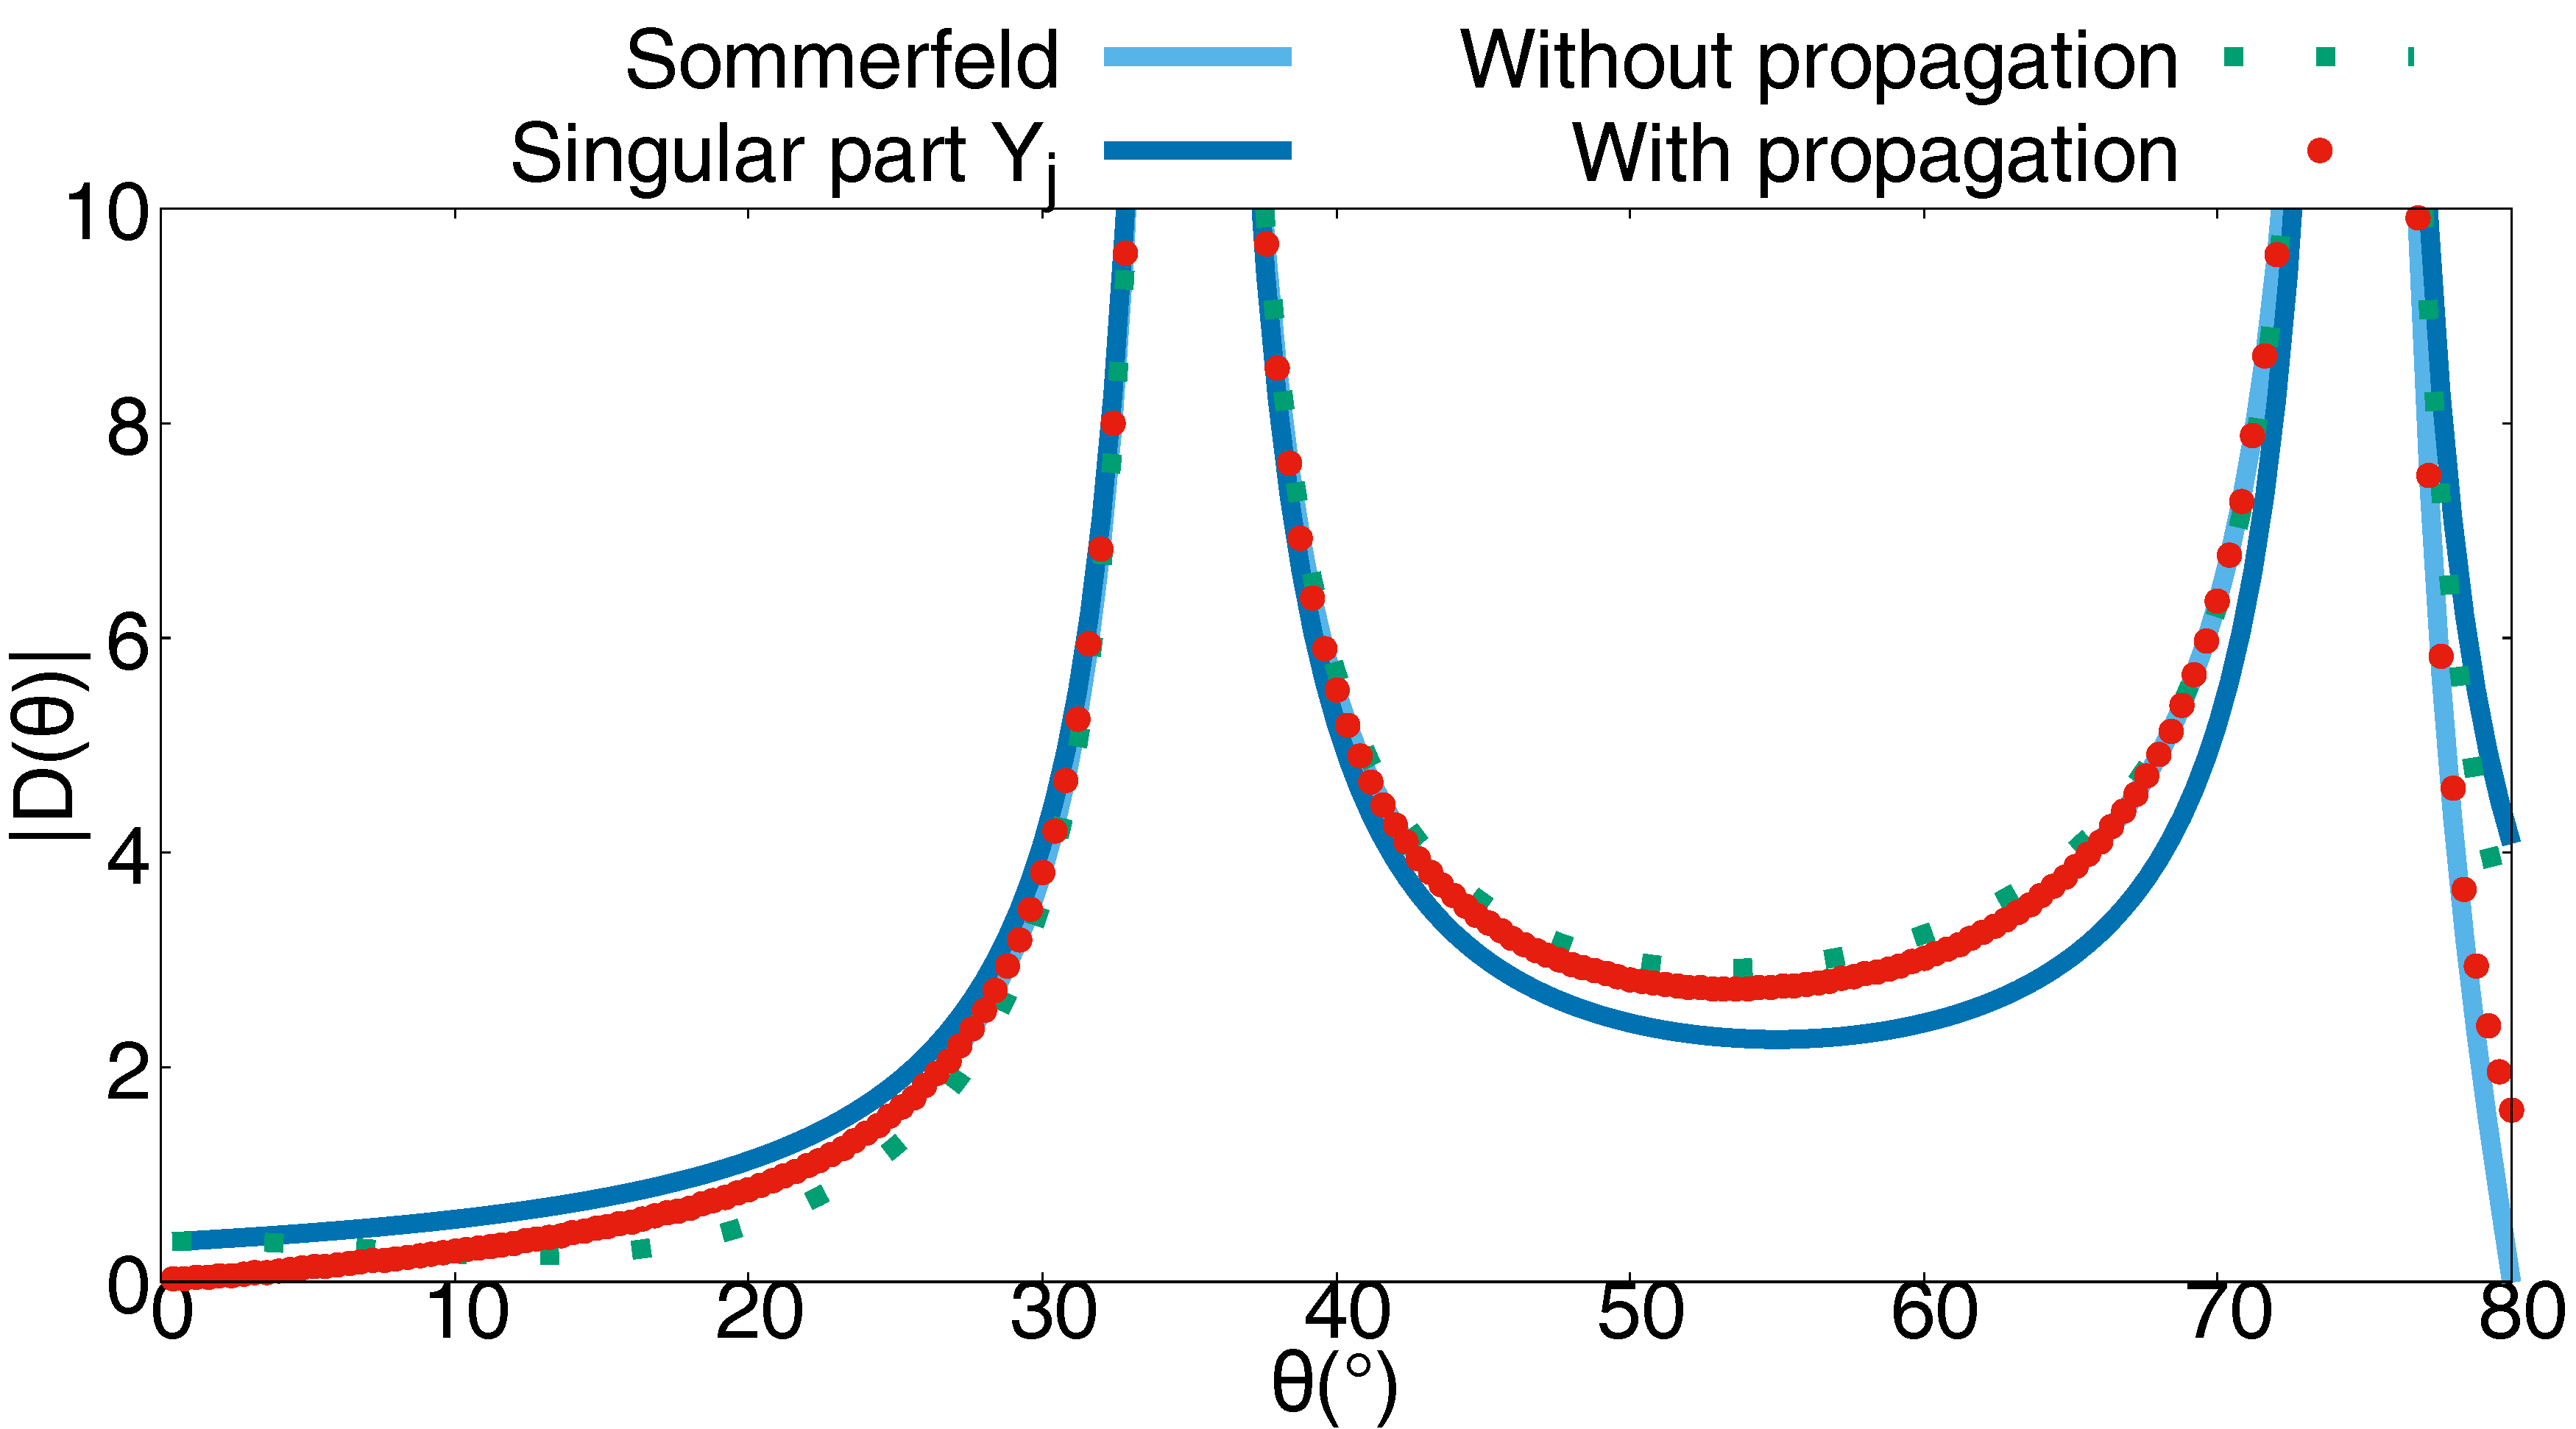
\includegraphics[width=\textwidth]{images/chapter2/Figure8a.pdf}
        \caption{$\varphi = 80^o$, $\theta_{\rm inc} = 55^o$}
        \label{chapter5:figure12a}
    \end{subfigure}
\begin{subfigure}[b]{0.49\textwidth}
        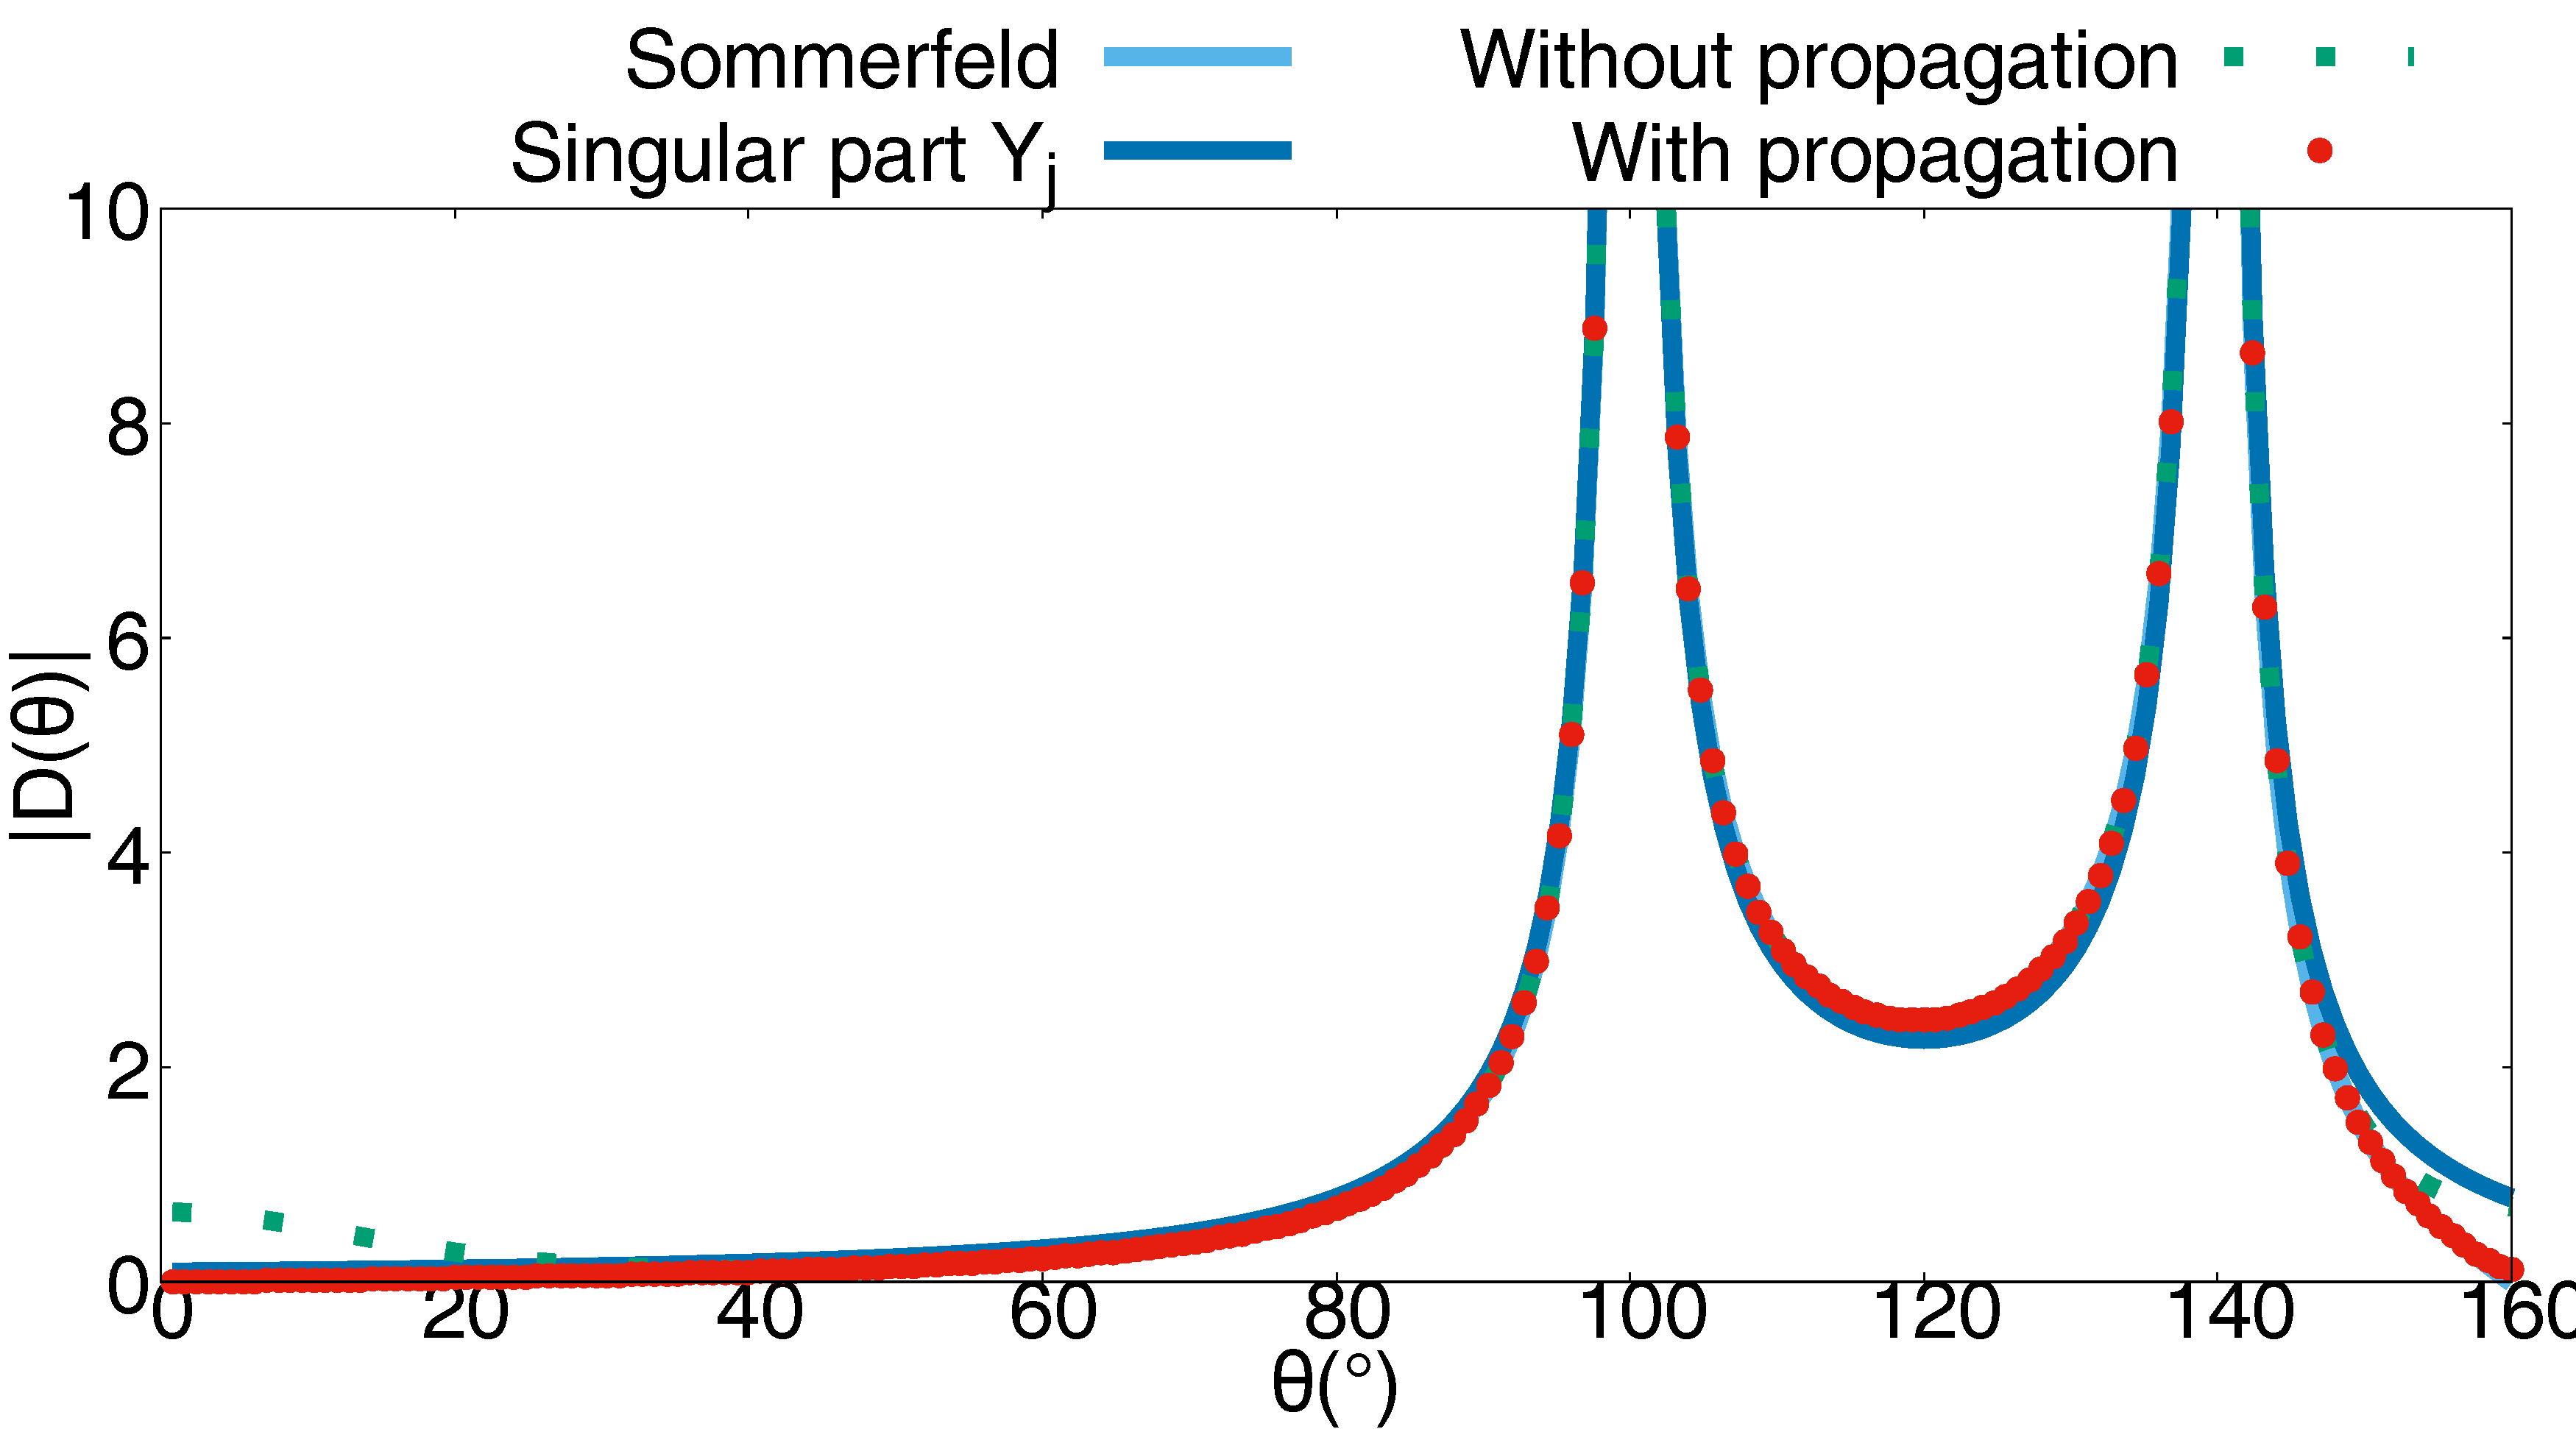
\includegraphics[width=\textwidth]{images/chapter2/Figure8b.pdf}
        \caption{$\varphi = 160^o$, $\theta_{\rm inc} = 40^o$}
        \label{chapter5:figure12b}
    \end{subfigure}
\\
~\\
\begin{subfigure}[b]{0.49\textwidth}
        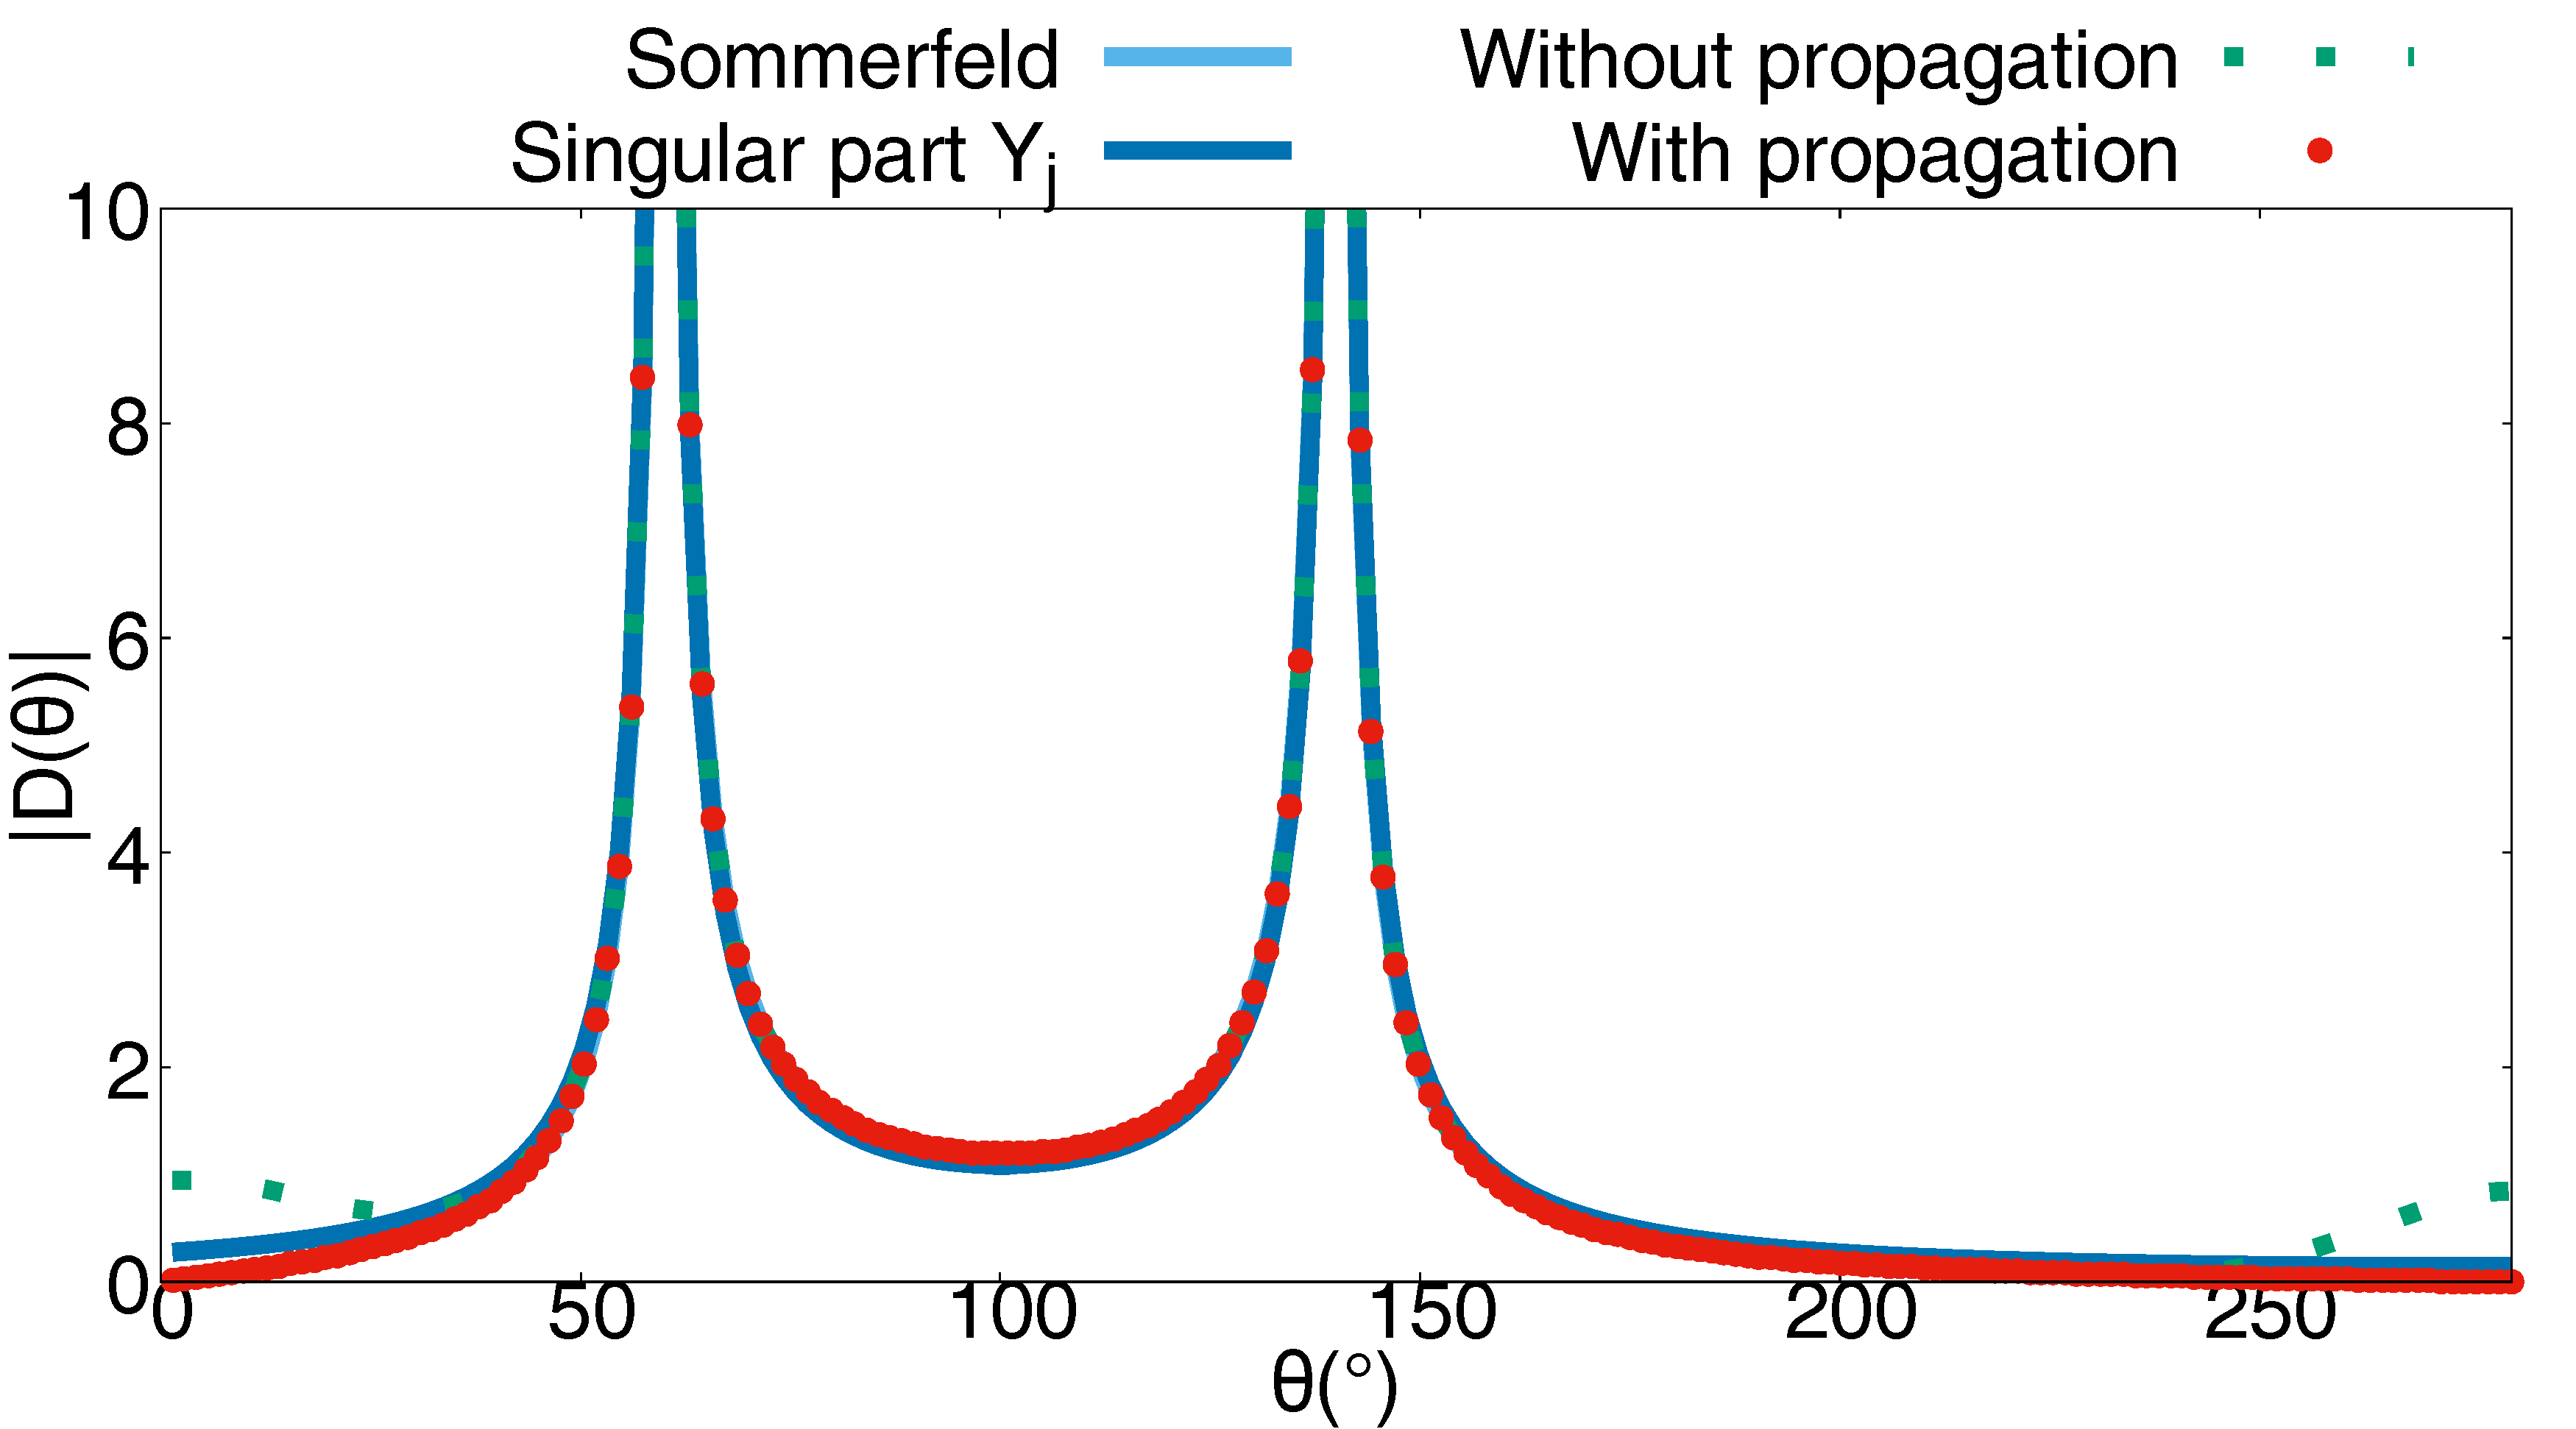
\includegraphics[width=\textwidth]{images/chapter2/Figure8c.pdf}
        \caption{$\varphi = 280^o$, $\theta_{\rm inc} = 240^o$}
        \label{chapter5:figure12d}
    \end{subfigure}
\begin{subfigure}[b]{0.49\textwidth}
        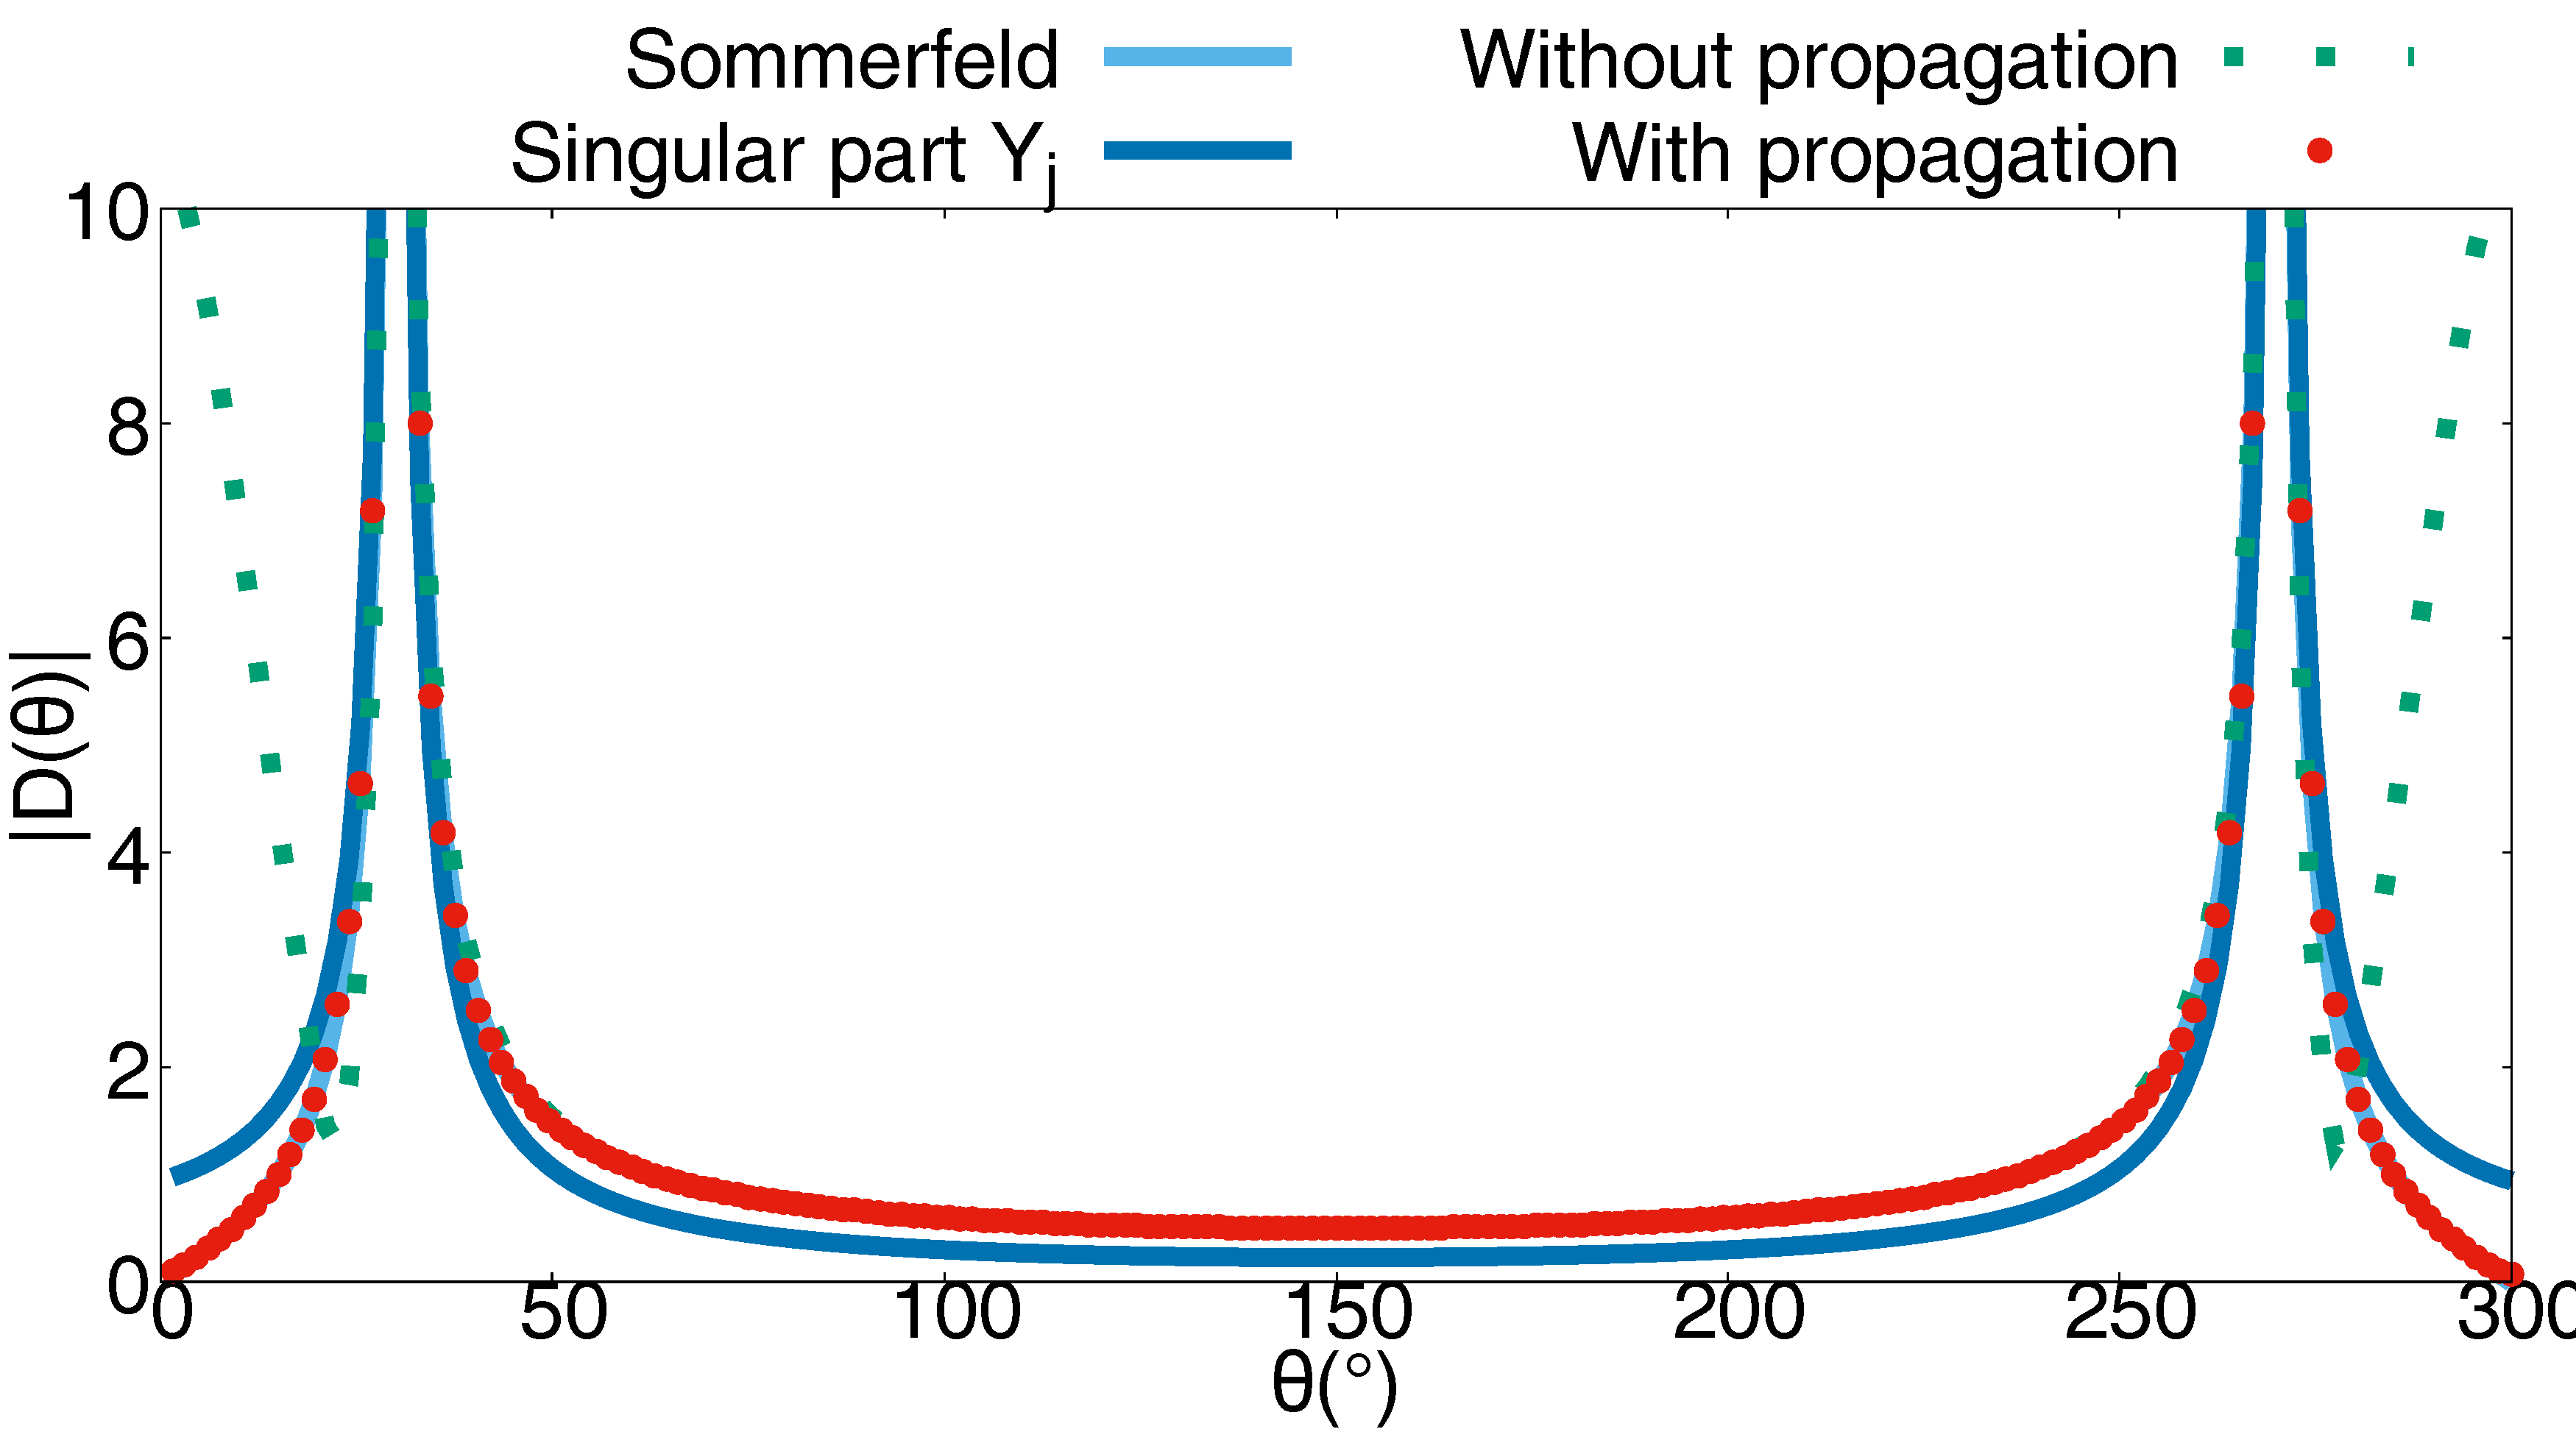
\includegraphics[width=\textwidth]{images/chapter2/Figure8d.pdf}
        \caption{$\varphi = 300^o$, $\theta_{\rm inc} = 150^o$}
        \label{chapter5:figure12c}
    \end{subfigure}
\caption
[Diffraction coefficient computed with the recursive formula of spectral functions and with the Sommerfeld method, in the case of Dirichlet boundary conditions]
{Diffraction  coefficient computed with the spectral functions and with the Sommerfeld method, in the case of Dirichlet boundary conditions.}
\label{chapter5:figure12}
\end{figure}

In the case of Neumann boundary conditions, a far-field evaluation of the diffraction, given by \eqref{GTDCoeff_SF} is compared to the analytic expression of the diffraction coefficient given by Sommerfeld \cite{Sommerfeld}. The GTD approximation of this coefficient is also given by Keller \cite{GTD} :
\begin{align}
\label{GTDCoeff_Neu}
D^{\rm (Neu)}(\theta) = \dfrac{e^{-i\frac{\pi}{4}}}{2\mathcal{N} \sqrt{2\pi}}  \, \left[ \cot \left( \dfrac{\pi + (\theta + \theta_{\rm inc})}{2\mathcal{N}} \right) + \cot \left( \dfrac{\pi - (\theta + \theta_{\rm inc})}{2\mathcal{N}} \right) \right.   \nonumber \\
\left. + \cot \left( \dfrac{\pi + (\theta - \theta_{\rm inc})}{2\mathcal{N}} \right) + \cot \left( \dfrac{\pi - (\theta - \theta_{\rm inc})}{2\mathcal{N}} \right) \right] 
\end{align}
The results are presented on Fig ~\ref{chapter5:figure13}.

\begin{figure}[h!]
\centering
\begin{subfigure}[b]{0.49\textwidth}
        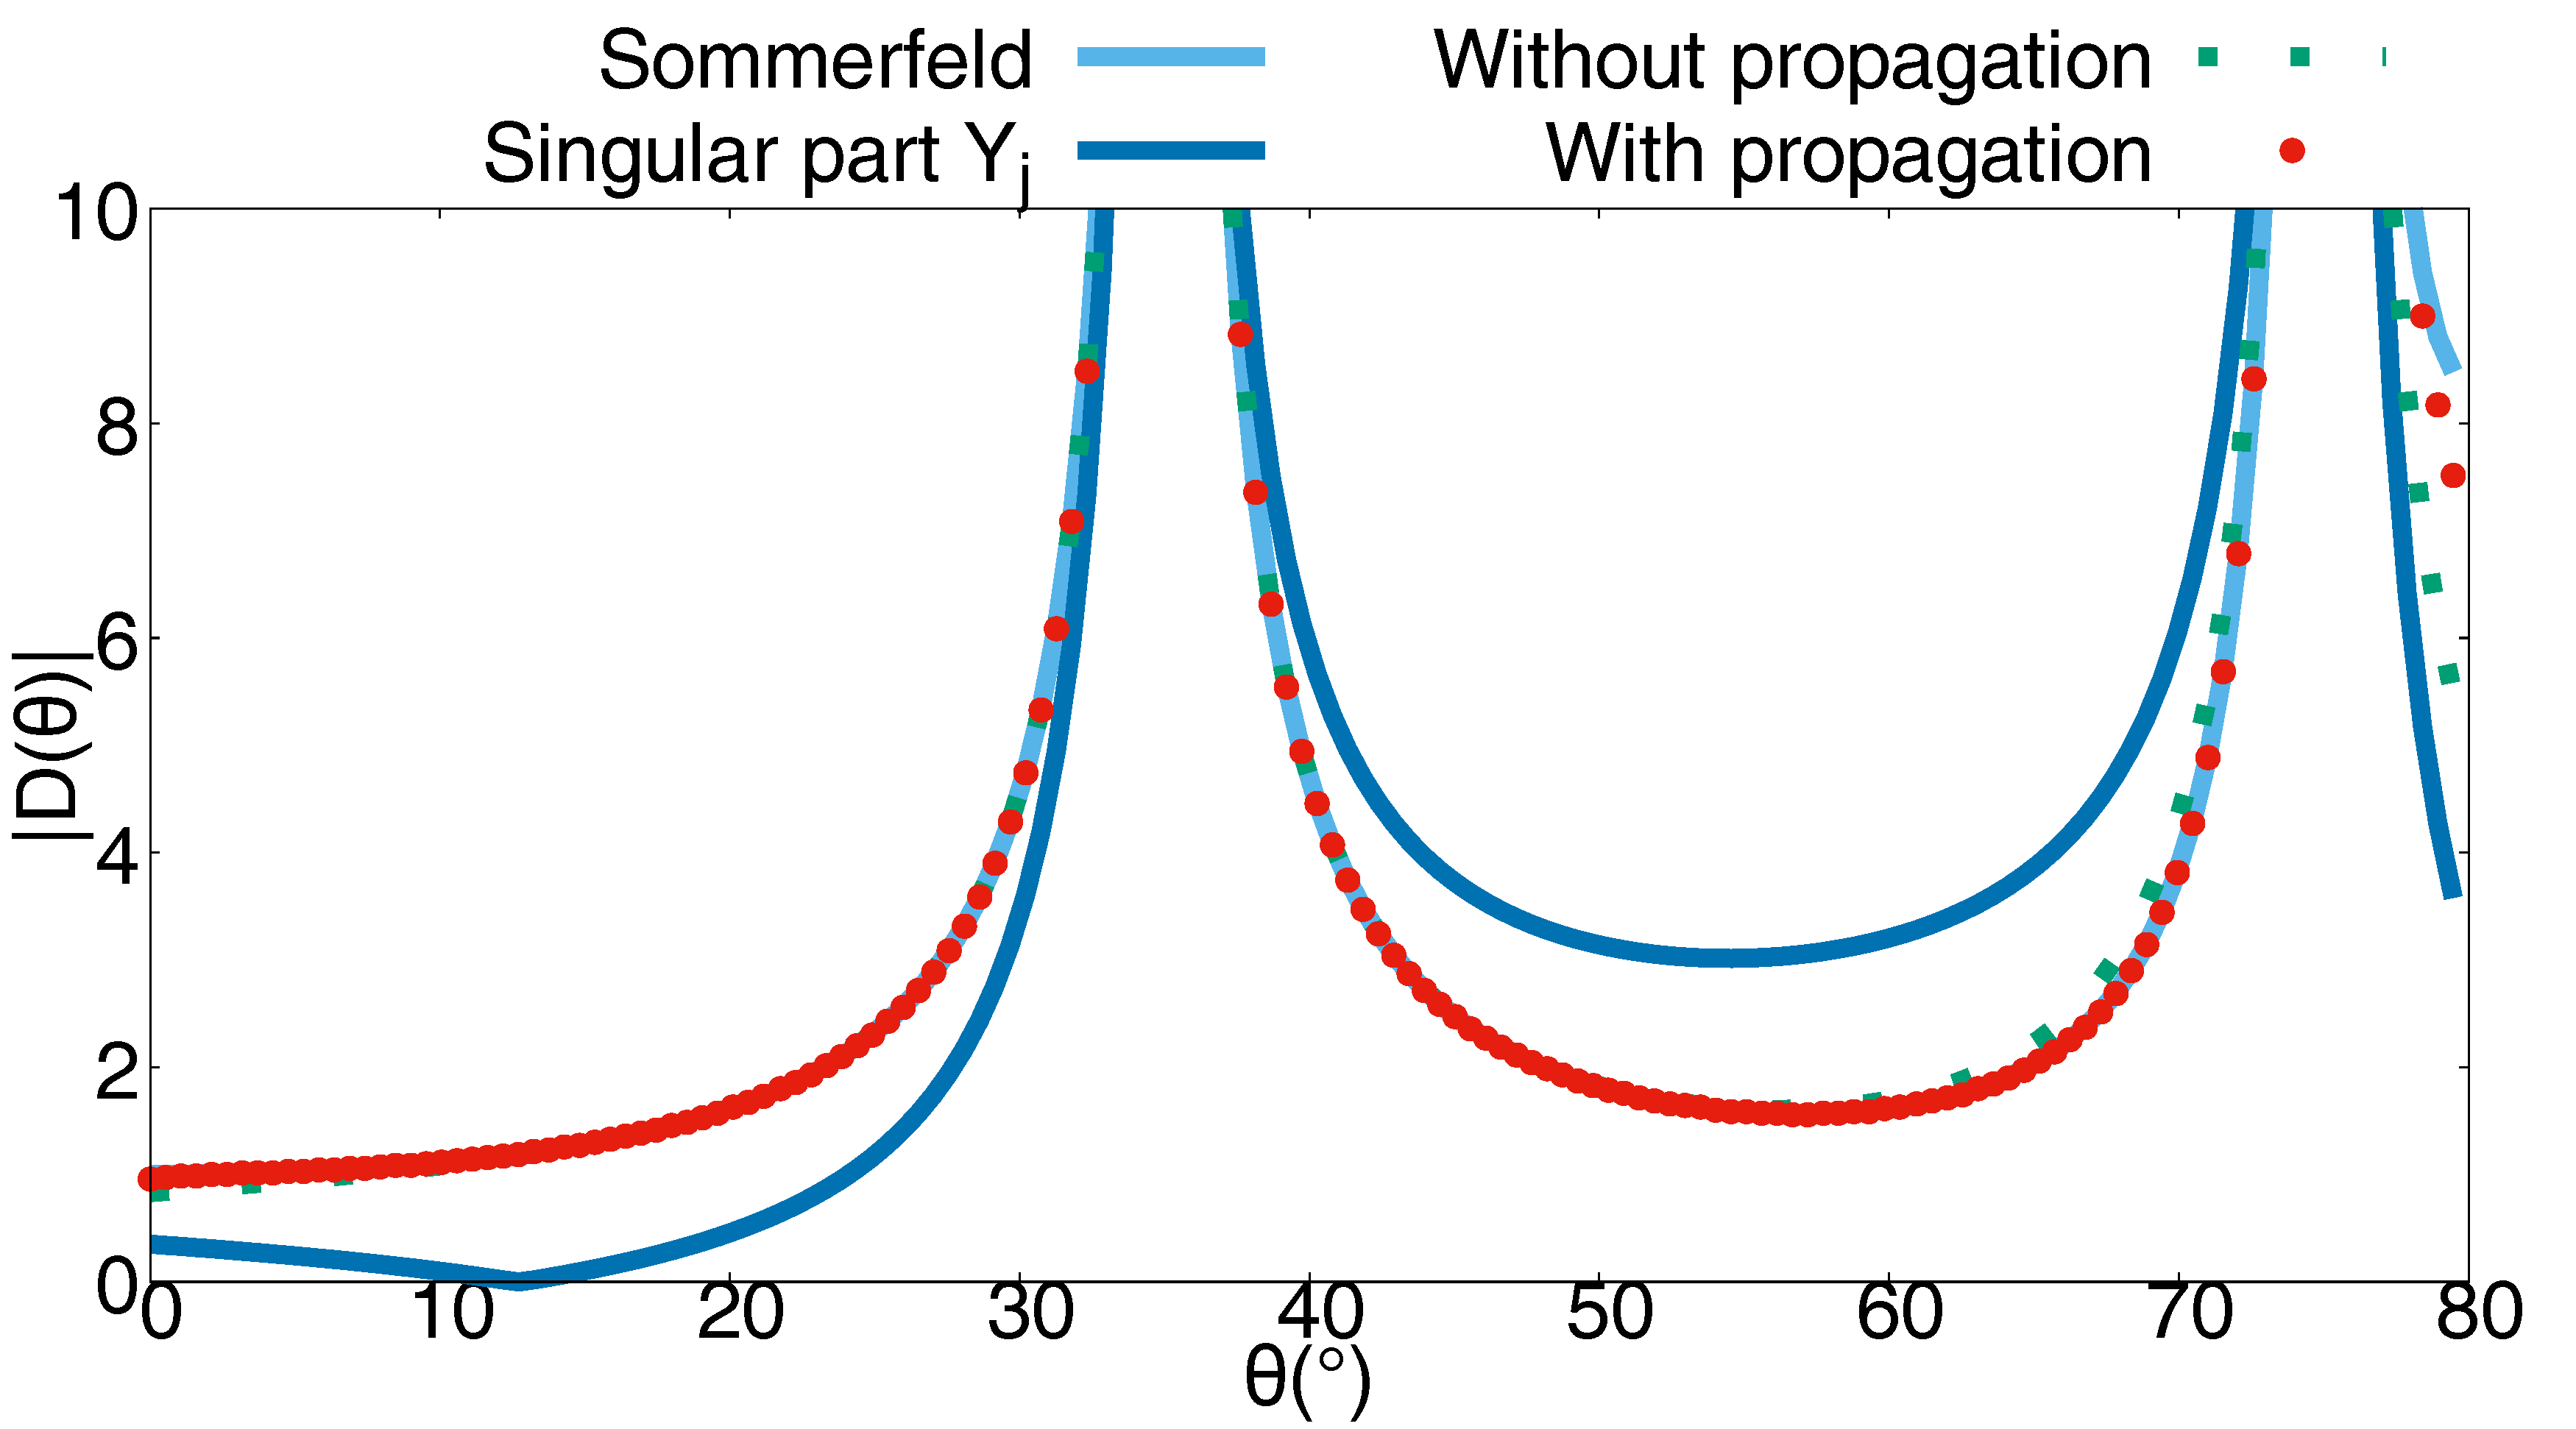
\includegraphics[width=\textwidth]{images/chapter2/Figure9a.pdf}
        \caption{$\varphi = 80^o$, $\theta_{\rm inc} = 55^o$}
        \label{chapter5:figure13a}
    \end{subfigure}
\begin{subfigure}[b]{0.49\textwidth}
        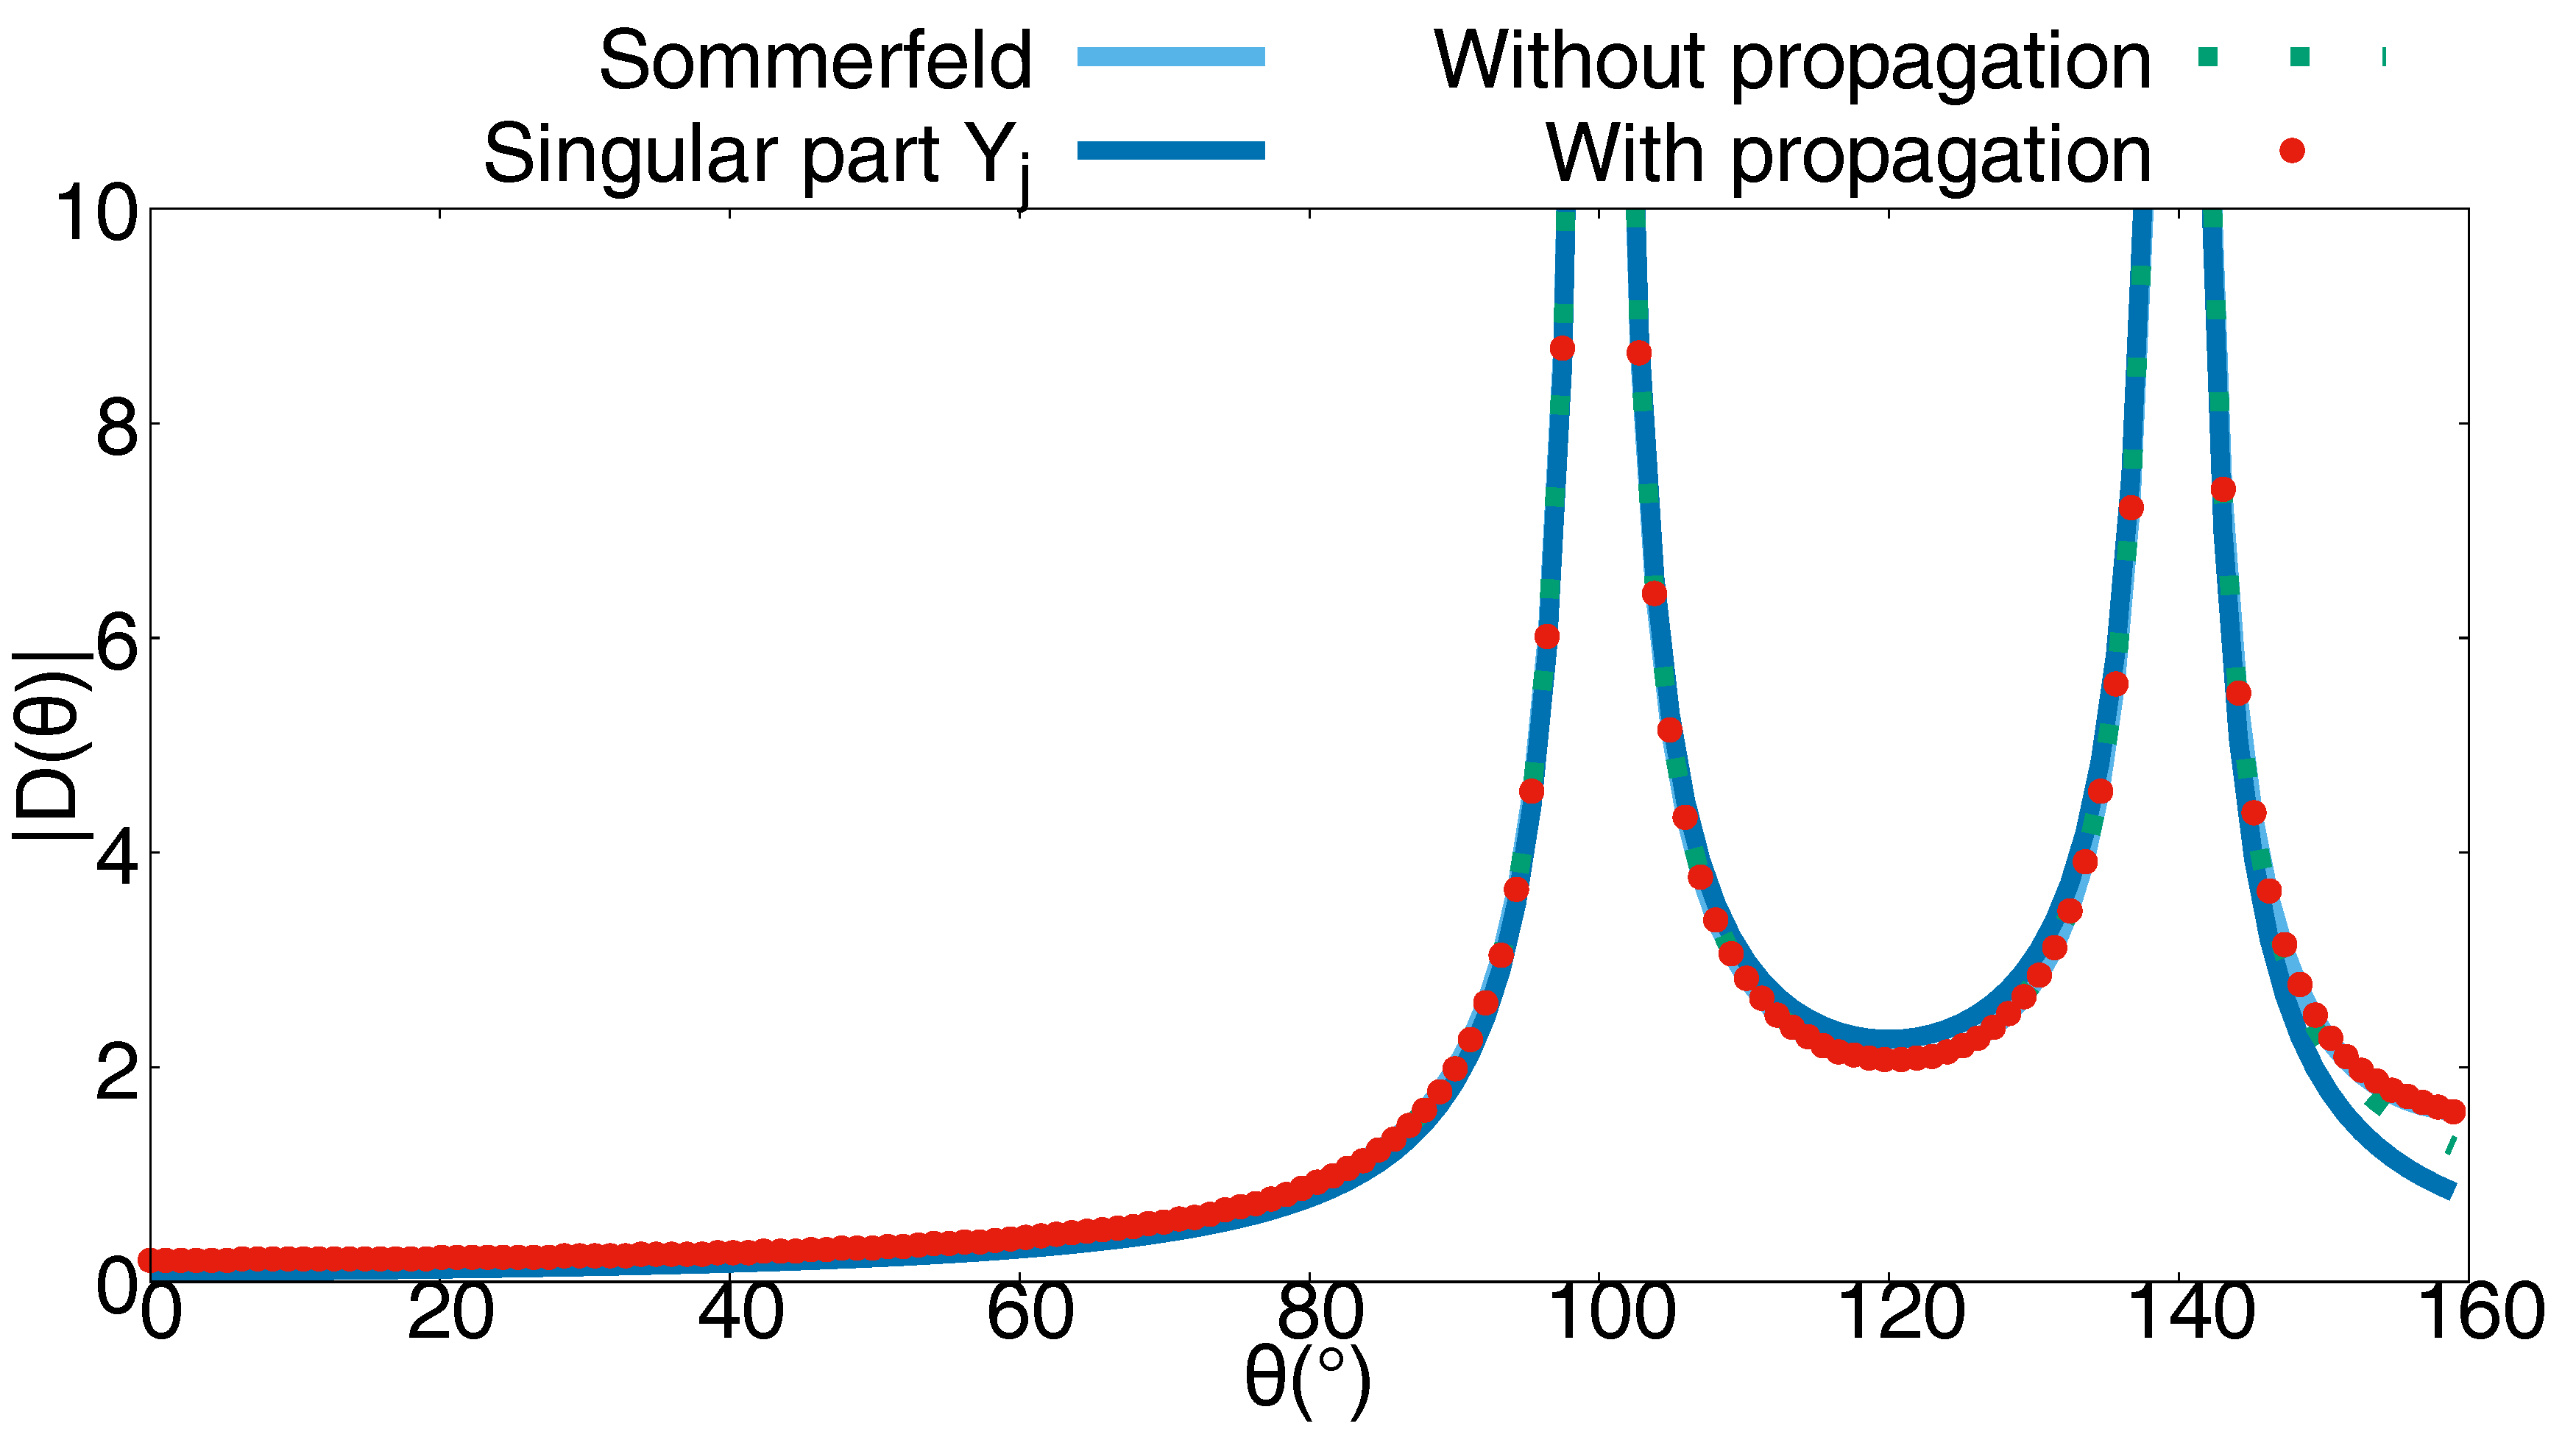
\includegraphics[width=\textwidth]{images/chapter2/Figure9b.pdf}
        \caption{$\varphi = 160^o$, $\theta_{\rm inc} = 40^o$}
        \label{chapter5:figure13b}
    \end{subfigure}
\\
~\\
\begin{subfigure}[b]{0.49\textwidth}
        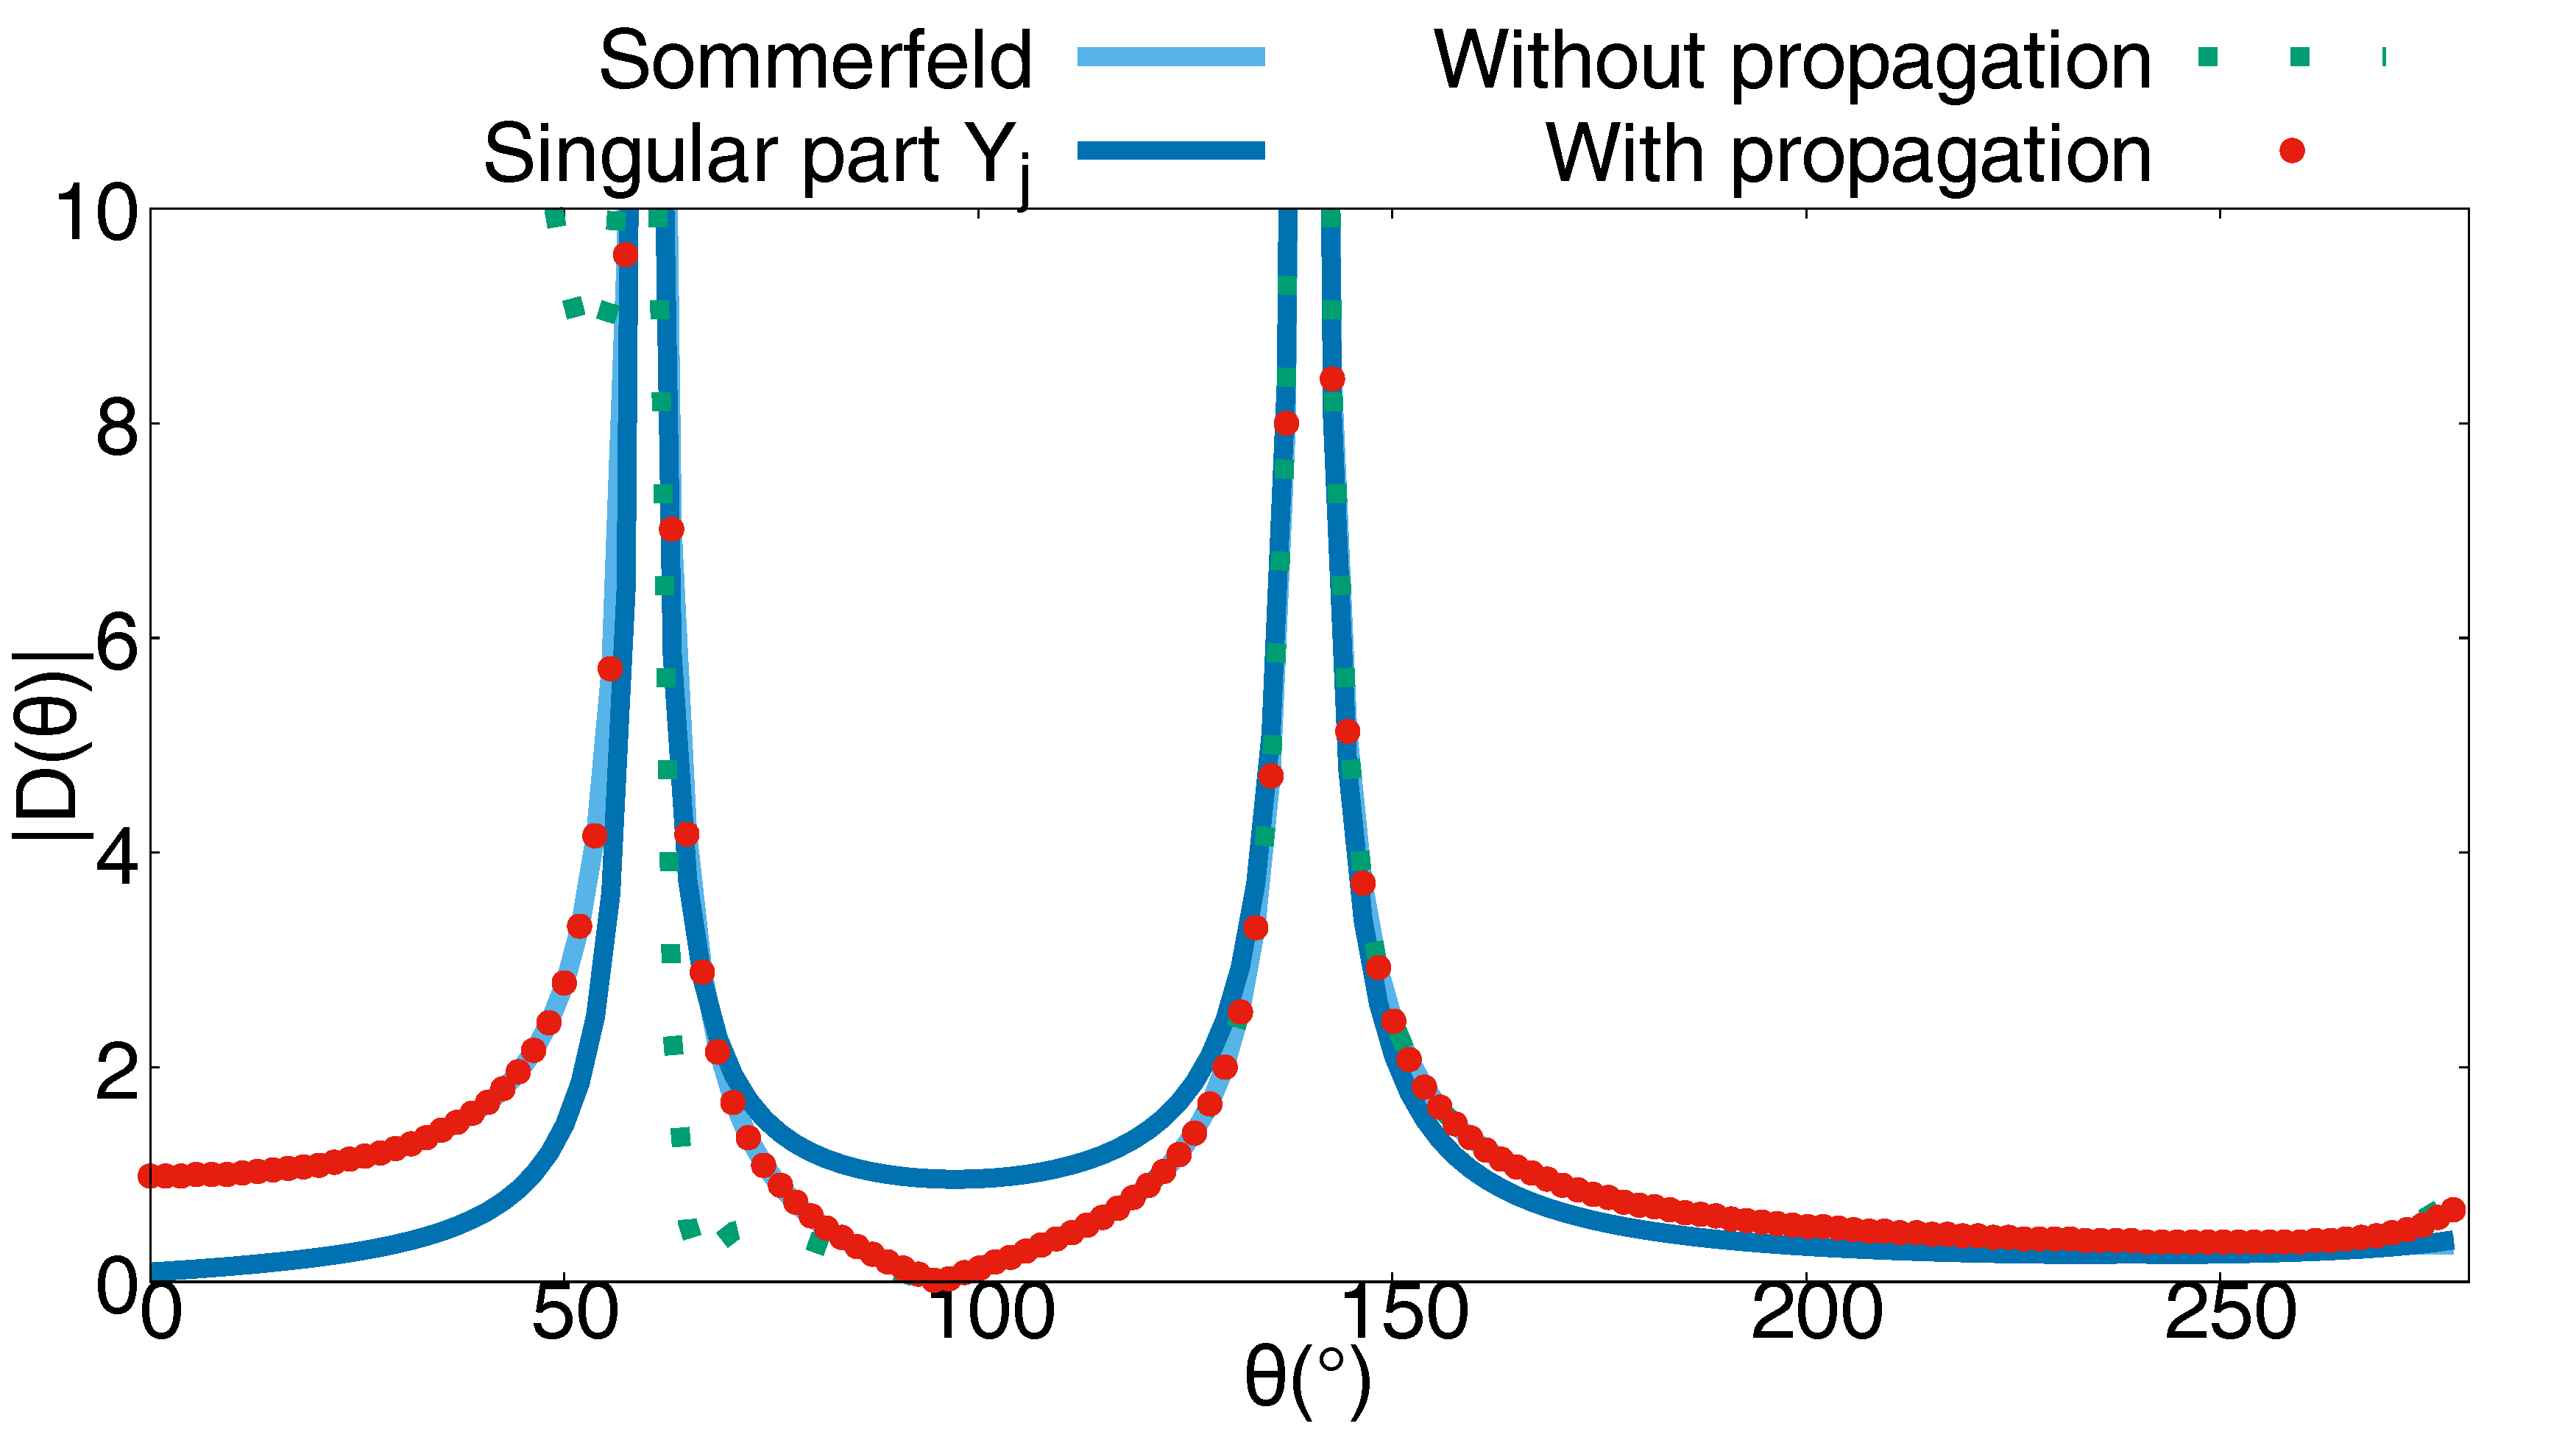
\includegraphics[width=\textwidth]{images/chapter2/Figure9c.pdf}
        \caption{$\varphi = 280^o$, $\theta_{\rm inc} = 240^o$}
        \label{chapter5:figure13d}
    \end{subfigure}
\begin{subfigure}[b]{0.49\textwidth}
        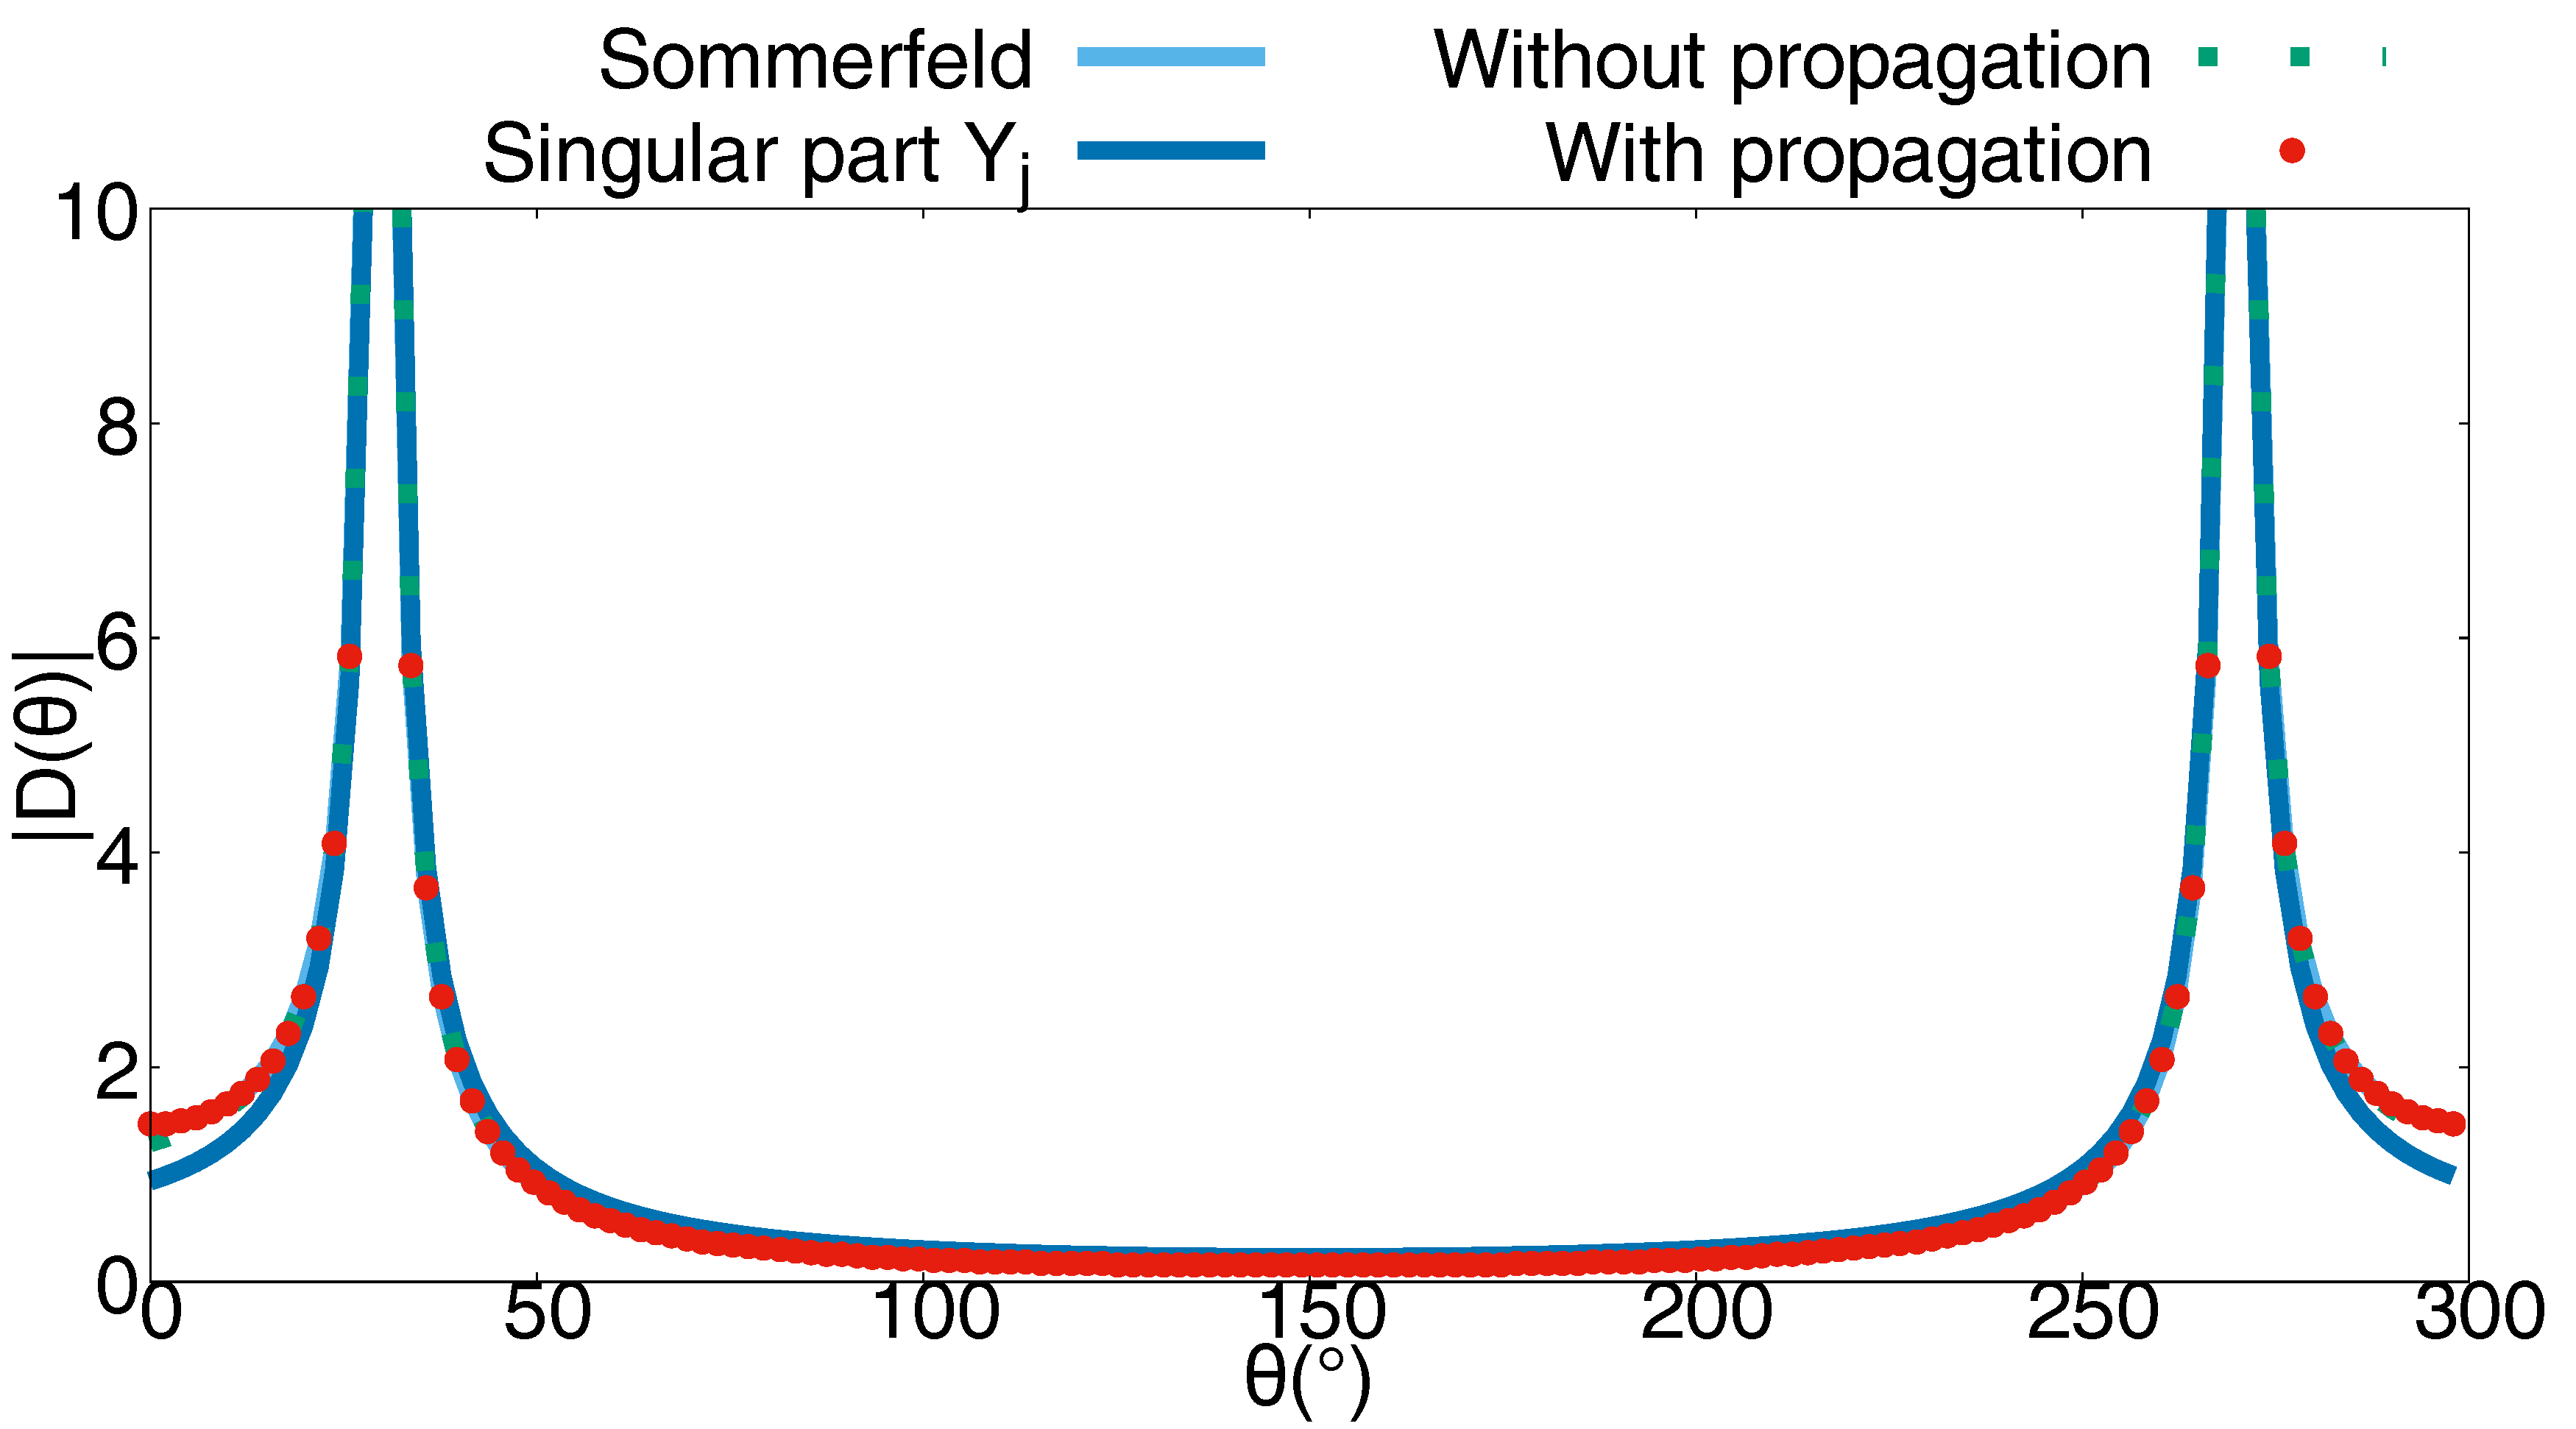
\includegraphics[width=\textwidth]{images/chapter2/Figure9d.pdf}
        \caption{$\varphi = 300^o$, $\theta_{\rm inc} = 150^o$}
        \label{chapter5:figure13c}
    \end{subfigure}
\caption
[Diffraction  coefficient computed with the recursive formula of spectral functions and with the Sommerfeld method, in the case of Neumann boundary conditions]
{Diffraction  coefficient computed with the spectral functions and with the Sommerfeld method, in the case of Neumann boundary conditions.}
\label{chapter5:figure13}
\end{figure}


 In each of these figures, the continuous light blue line represents the modules of the diffraction coefficients obtained using the Sommerfeld integral method, the continuous dark blue line represents those obtained using the Spectral function singular part $Y_j$ alone, the short-dashed green line represents those obtained using the Spectral functions method without propagation of the solution and the red circles represent those obtained using the spectral functions method with propagation of the solution described in paragraph \ref{propag_sol}.

On Figs.~\ref{chapter5:figure12a},~\ref{chapter5:figure12b},~\ref{chapter5:figure13a} and ~\ref{chapter5:figure13b} the wedge angles are lower than $\pi$ and on figs.~\ref{chapter5:figure12c},~\ref{chapter5:figure12d},~\ref{chapter5:figure13c} and ~\ref{chapter5:figure13d} the wedge angles are greater than $\pi$. In all cases, it appears clearly that both the regular part of the solution and the recursive method are necessary to obtain optimal results. When both of these are included, diffraction coefficients obtained with Spectral functions are close to those of the Sommerfeld method. In addition, the run time to evaluate the diffraction coefficients in 250 different observation points, in each of the presented configurations, using an Intel(R) Xeon(R) CPU E3-1240 v3 is under 0.1 seconds for both methods. 

\section*{Conclusion}
The spectral functions method is developed here to model diffraction of an acoustic wave by stress-free soft or hard wedges. The main steps of the method have been summarized in section \ref{C2:summary}. The diffraction coefficient obtained using the spectral functions method has been compared to the analytic one obtained from the asymptotic evaluation of the Sommerfeld integral. The numerical results obtained thanks to the spectral functions method are very close to those given by the analytical solution and the result is obtained at a very low computational cost. This proves the applicability and feasibility of the spectral functions method, as well as its efficiency and its precision. It may therefore be extended to more complex wedge diffraction cases such as 2D and 3D elastic wave diffraction, as will be shown in the following chapters. 
